\documentclass[onecolumn, draftclsnofoot,10pt, compsoc]{IEEEtran}
\usepackage{graphicx}
\usepackage{subcaption}
\usepackage{url}
\usepackage{setspace}
%\usepackage{hyperref}
\usepackage{setspace}
\usepackage{indentfirst}
\usepackage{listings}

\usepackage{geometry}
\geometry{textheight=9.5in, textwidth=7in}

% 1. Fill in these details
\def \CapstoneTeamName{		100k Challenge CS}
\def \CapstoneTeamNumber{		42}
\def \GroupMemberOne{			Michael Elliott}
\def \GroupMemberTwo{		 	Sam Hudson}
\def \GroupMemberThree{			Glenn Upthagrove}
\def \CapstoneProjectName{		100K Spaceport America Demonstration Rocket Project }
\def \CapstoneSponsorCompany{	School of MIME}
\def \CapstoneSponsorPerson{		Nancy Squires}

% 2. Uncomment the appropriate line below so that the document type works
\def \DocType{		%Technology Review
				%Requirements Document
				%Technology Review
				%Design Document
				%Progress Report
				Final Report
				}
			
\newcommand{\NameSigPair}[1]{\par
\makebox[2.75in][r]{#1} \hfil 	\makebox[3.25in]{\makebox[2.25in]{\hrulefill} \hfill		\makebox[.75in]{\hrulefill}}
\par\vspace{-12pt} \textit{\tiny\noindent
\makebox[2.75in]{} \hfil		\makebox[3.25in]{\makebox[2.25in][r]{Signature} \hfill	\makebox[.75in][r]{Date}}}}
% 3. If the document is not to be signed, uncomment the RENEWcommand below
%\renewcommand{\NameSigPair}[1]{#1}

%%%%%%%%%%%%%%%%%%%%%%%%%%%%%%%%%%%%%%%
\begin{document}
\begin{titlepage}
    \pagenumbering{gobble}
    \begin{singlespace}
    	
\includegraphics[height=4cm]{coe_v_spot1} %HERE
        \hfill 
        % 4. If you have a logo, use this includegraphics command to put it on the coversheet.
        %\includegraphics[height=4cm]{CompanyLogo}   
        \par\vspace{.2in}
        \centering
        \scshape{
            \huge CS Capstone \DocType \par
            {\large\today}\par
            \vspace{.5in}
            \textbf{\Huge\CapstoneProjectName}\par
            \vfill
            {\large Prepared for}\par
            \Huge \CapstoneSponsorCompany\par
            \vspace{5pt}
            {\Large\NameSigPair{\CapstoneSponsorPerson}\par}
            {\large Prepared by }\par
            Group\CapstoneTeamNumber\par
            % 5. comment out the line below this one if you do not wish to name your team
            %\CapstoneTeamName\par 
            \vspace{5pt}
            {\Large
                \NameSigPair{\GroupMemberOne}\par
                \NameSigPair{\GroupMemberTwo}\par
                \NameSigPair{\GroupMemberThree}\par
            }
            \vspace{20pt}
        }
        \begin{abstract}
        % 6. Fill in your abstract    
	The software suite developed for the American Institute of Aeronautics and Astronomic (AIAA) Spaceport America 100k Rocketry challenge for Oregon State University shall track a rocket as it flies. The resulting data will be used to both visualize the flight path and collect the rocket upon return to the surface. The software shall collect, filter, log, and visualize the data. This document describes the design of these systems. 
        \end{abstract}     
    \end{singlespace}
\end{titlepage}
\newpage
\pagenumbering{arabic}
\tableofcontents
% 7. uncomment this (if applicable). Consider adding a page break.
%\listoffigures
%\listoftables
\clearpage

% 8. now you write!
\section {Introduction}
The project completed by computer science group 42 over the 2017 and 2018 school year was the creation of software that could track the flight of a rocket for the Oregon State University High Altitude Rocket Team. The project was requested on behalf of the Oregon State University college of Mechanical, industrial, and Manufacturing Engineering (MIME). The client who oversaw the interdisciplinary team and served as important advisor was Dr. Nancy Squires.\par
The Computer Science team consisted of three students Michael Elliott, Samuel Hudson, and Glenn Upthagrove. Each member took primary responsibility for portions of the project that best fit their skill set and experience. Michael Elliott was the primary programmer for the mathematically intensive Kalman filter and data interpolation which aided in cleaning the noise out of the data caused by the stresses of flight. Samuel Hudson was in charge of the database and the web application which displayed the final data to the user in a more accessible manner. Glenn Upthagrove took responsibility for the data handling and trace, which was the collection and conversion of raw data and the secondary display of the final data to the user in a 3D space.
\section {Requirments Document}
\subsection{Abstract}
The Transmission protocol and Kalman filter we shall maximize data integrity. The
Ground Station shall collect the data in near real time, and display this data to the screen at a
constant refresh rate. The visualization will be human readable and display the best known
approximation of the position of the rocket. The following details the features and
expectations of the software we shall be developing.\par
\subsection{Introduction}
\subsubsection{Purpose}
This document shall serve going forth as a description of the requirements and
expectations of the software created by the computer science sub team for the 100k rocketry
challenge.
\subsubsection{Scope}
The software created by this sub-team shall, in conjunction with electrical sub-
team, create a transmission protocol and Kalman filter to transmit and receive the data as
accurately as possible. The data shall be stored on the ground station. There shall also be a
visualization that can present this data to the user. This implies:
 \begin{enumerate}
    \item The rocket can be tracked and recovers.
    \item The highest altitude can be recorded.
    \item The user will be able to view the data at a rate that is readable.
 \end{enumerate}
\subsubsection{Definitions and Acronyms}
Blackout: A long period where no data is recovered. \par
Corruption: When data in transmission changes value due to interference. \par
Data: Measurements of importance. \par
GS: Ground Station, a computer on the ground used during the flight. \par
GUI: Graphical User Interface. A visual interface with the software. \par
JSON: JavaScript Object Notation. A way of annotating data. \par
Kalman Filter: A system which uses both data and an ideal model to make a best estimate. \par
KATE: A software package for making announcements at certain altitudes. \par
Noise: Improper readings from sensors due to its constraints. \par
Packet: a complete set of data that is transmitted. \par
Packet Loss: When a packet does not reach the destination. \par
Protocol: The system for packaging and transmitting the telemetry data. \par
Serial: Data transferred sequentially over a single data line. \par
Telemetry: The data used for tracking the data. \par
\subsubsection{Overview}
The remainder of this document describes in more detail the aspects and
requirements of the software. This shall involve the interaction between our software and the
other aspects of the project. The following section, \textit{Overall Description}, shall give a broad
description of what our software shall do and the factors we must work with. The last section,
\textit{Specific Requirements}, shall put forth in detail the exact expectations of the software we shall
deliver.
\subsection{Overall Description}
\subsubsection{Product Perspective}
The transmission protocol shall transmit the data from the rocket to
the GS as accurately as possible. There shall also be a Kalman filter that will help to keep the
data accurate beyond the capabilities of the protocol and the noise associated with the
sensors. The GS will receive data via a wireless interface with the rocket. The data will be
transmitted in a serial fashion. The ground station will not be connected to the Internet, and
shall be in communication only with the rocket. The data the GS receives from the rocket shall
be stored, and used to update the visualization shown to the user.
\subsubsection{Product Functions: The software shall provide several features}
 \begin{enumerate}
    \item The data shall be collected and stored for later use.
    \item The data shall be displayed to the user in near real time.
    \item The data can be used later to create a 3D trace of the flight path.
 \end{enumerate}
\subsubsection{User Characteristics}
The GS shall be used only by people associated with this
challenge, and thus have some level of technical knowledge. The visualization and 3D trace
should, however, also easily readable by anyone.
\subsubsection{Constraints}
 \begin{enumerate}
    \item Due to the altitude the rocket shall theoretically reach, there is a significant chance that
packet loss and blackout could occur.
    \item Due to the body of the rocket being in large part carbon fiber, there is a chance this could
also cause packet loss.
    \item The rocket has limited processing power.
    \item The ground station will also not be very powerful.
 \end{enumerate}
\subsubsection{Assumptions and Dependencies}
We assume the rocket shall be using a Telemega chip. We also assume that the GS will be
based off of a Raspberry Pi, running a distortion of Linux.
\subsubsection{Apportioning of Requirements}
There is a gantt chart in figure 1. This outlines the time line for our software from now until the
test launch. Our software must be at a stable state by the test launch so it can be used to full
effect at that time.
\subsection{Specific Requirements}
\subsubsection{Protocol Requirements} The protocol will be able, as long as there is a connection, to
transmit a full set of telemetry data at least once per second. The packets shall also be
packaged in a JSON or similar format.

\subsubsection{GS Requirements}
The GS shall be able to display a visualization and update the
visualization once per second.
\subsubsection{Visualization Requirements}
The visualization will be human readable. This will be
defined by at least 6 out of 10 people asked to review the visualization agreeing. These
people will not be EECS majors, nor in similar fields. There will be an update once per
second. This will make the visualization near real time.
\subsubsection{3D Trace Requirements}
The trace shall be able to read the recorded data after the flight
and display the flight path in 3D space.
\subsubsection{Near Real Time 3D Trace (Stretch Goal)}
The trace can display the flight path in near
real time as the data is received on the GS.
\subsubsection{KATE Integration (Stretch Goal)}
We shall integrate KATE into our GS.
%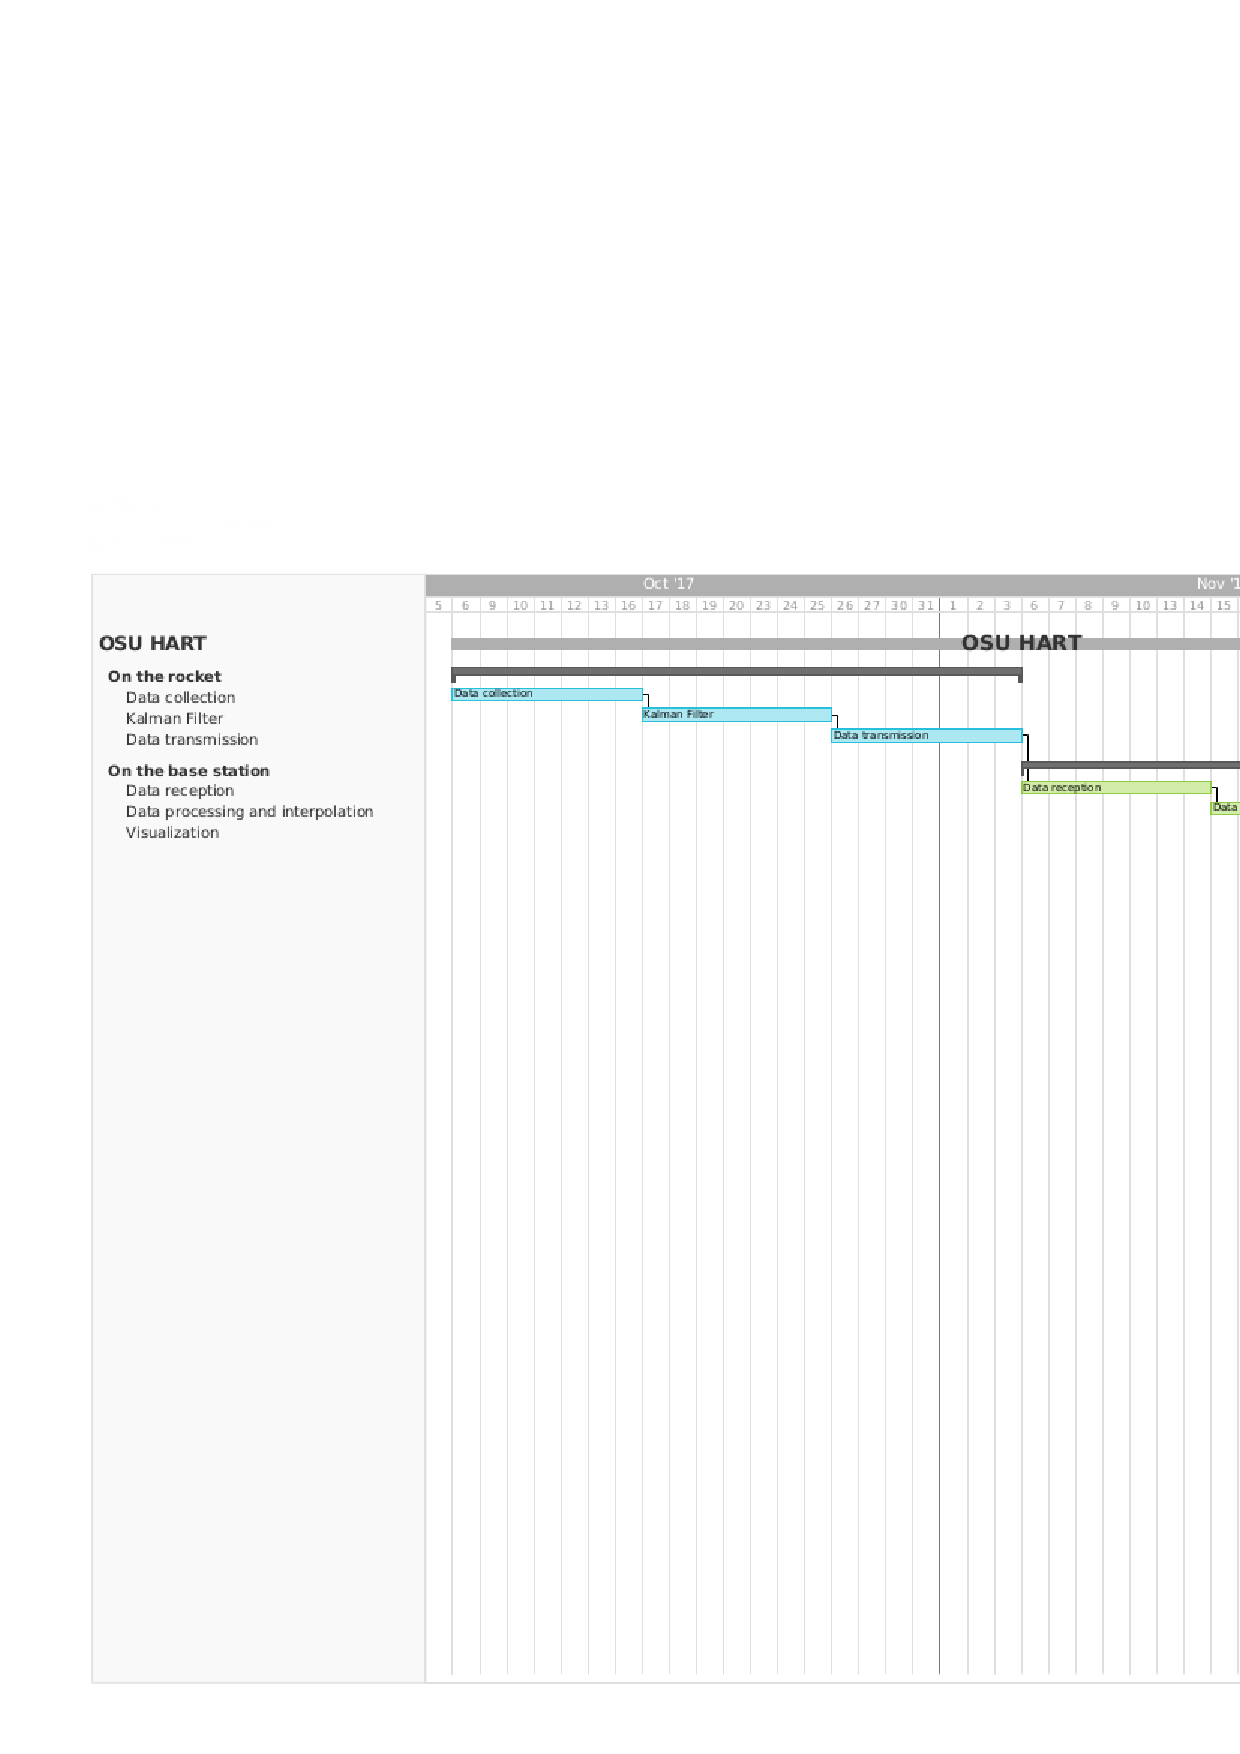
\includegraphics[width=\textwidth,height=\textheight]{gantt}
%HERE

\begin{figure}[h]
    \centering
%    \begin{subfigure}[Figure 1a]{0.3\textwidth}
        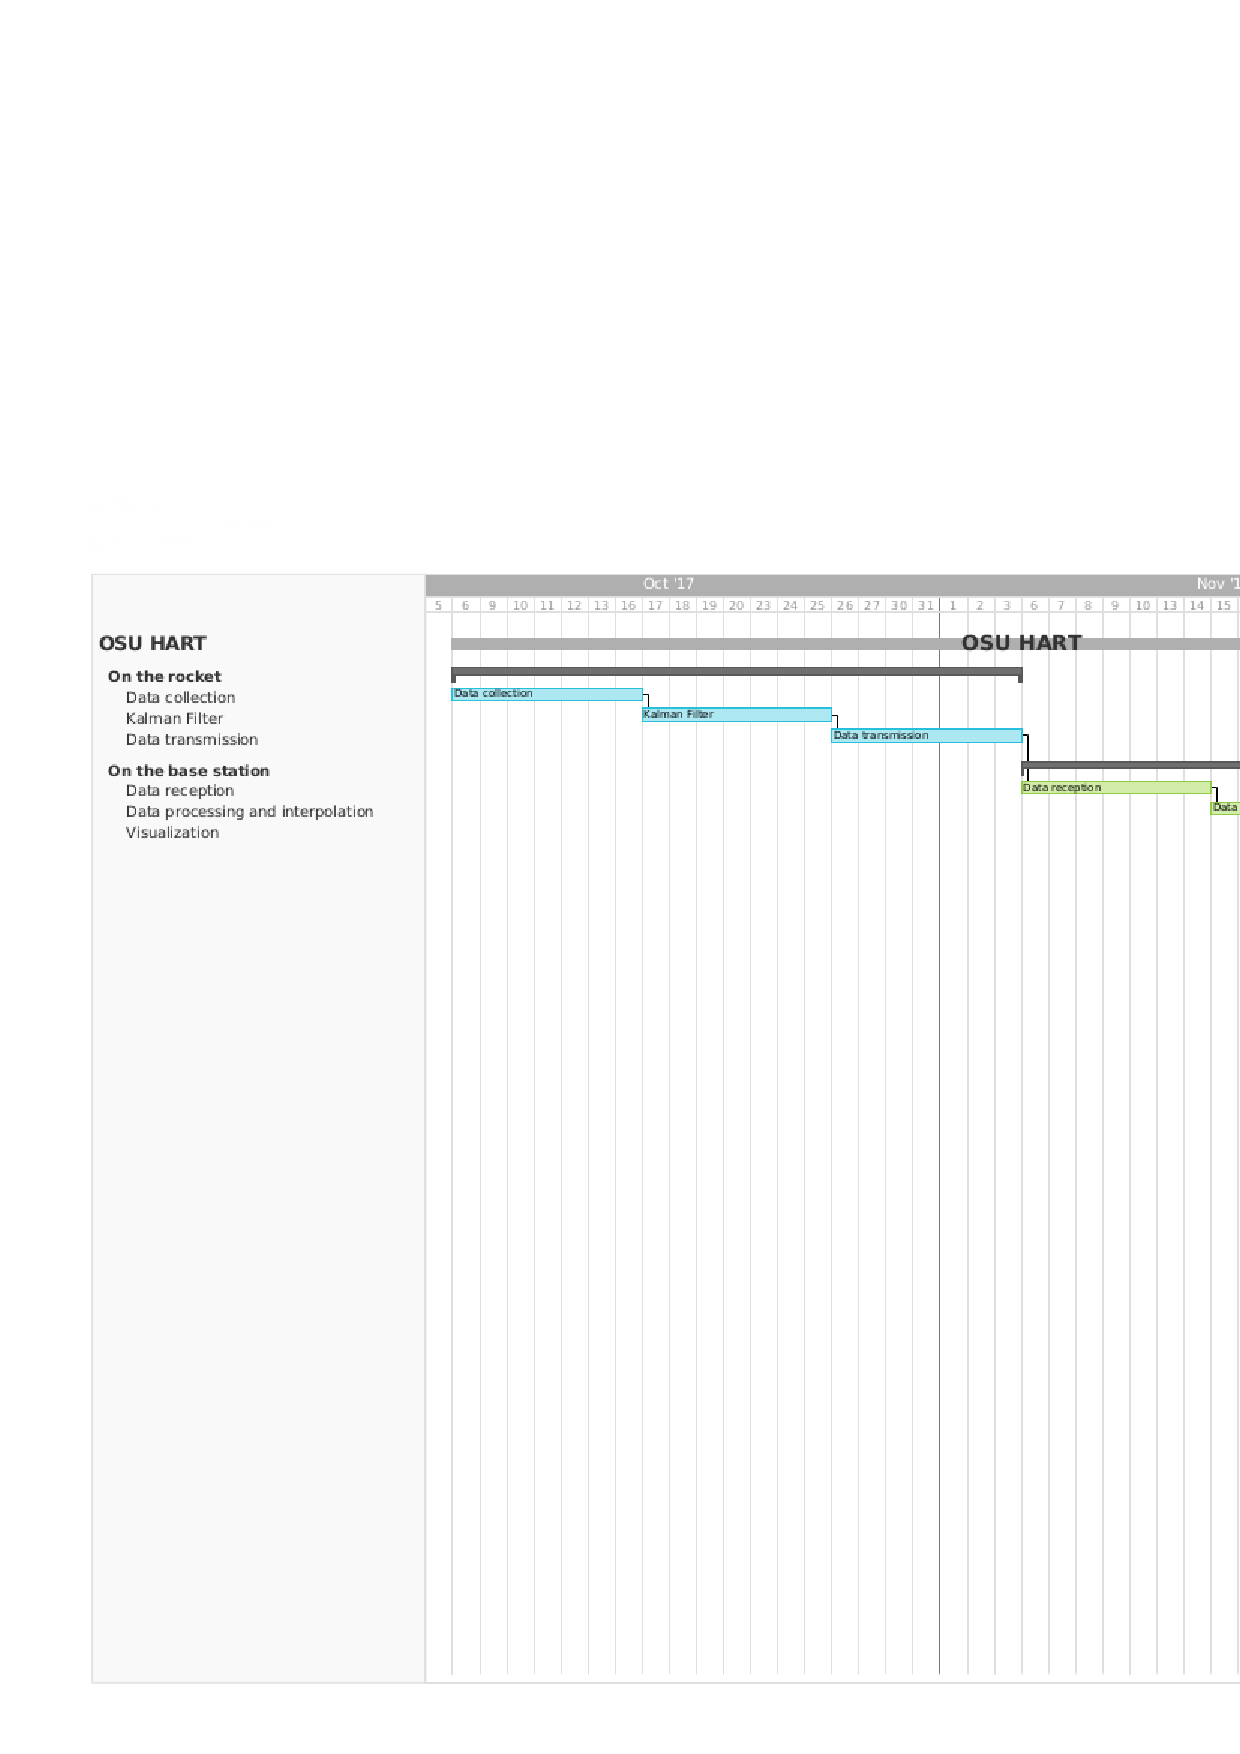
\includegraphics[width=16cm]{gantt}
        \caption{The original Gantt chart}
        \label{fig:gantt}
%    \end{subfigure}
\end{figure}

\section{Updated Gantt Chart}
\begin{figure}[h]
    \centering
%    \begin{subfigure}[Figure 1a]{0.3\textwidth}
        \includegraphics[width=16cm]{ganttfinal}
        \caption{The final Gantt chart}
        \label{fig:ganttfinal}
%    \end{subfigure}
\end{figure}


\section {Design Document}
\subsection {Abstract}
The software suite developed for the American Institute of Aeronautics and Astronomic (AIAA) Spaceport America 100k Rocketry challenge for Oregon State University shall track a rocket as it flies. The resulting data will be used to both visualize the flight path and collect the rocket upon return to the surface. The software shall collect, filter, log, and visualize the data. This document describes the design of these systems.
\subsection {Overview}
\subsubsection {Scope}
The following shall describe the design for the software that shall track the high altitude rocket for Oregon State University. The software shall primarily be running on the rocket, and a ground station. The data shall be collected from the sensors on the rocket, and begin a journey down a software pipeline towards final display, which will filter the data, package it, transmit it, collect it, covert it to a readable format, log it, and display it in both 2D and 3D displays. 
\subsubsection {Purpose} 
This software suit is intended to give reliable tracking of a rocket in flight, and graphically represent this data to the user. The general goals being the safe recovery of the rocket after it has completed its flight and come to rest. This is necessary as the rocket in this case shall go well outside of visible range, and the use of automated tracking shall be essential to the recovery. 
\subsubsection {Intended Audience}
The intended audience for this document are the engineering students responsible for the creation and use of the rocket, as well as their advisors. All involved are educated individuals, with a wide variety of expertise. Some have a very solid understanding of computer science whilst other have very different ares of expertise. This document provides sufficient description and detail for the most familiar of these stakeholders to understand most of the underlying systems, and a high enough view of the project and the connections for the readers of different background to still understand the purpose and general concepts behind the system. 
\subsection{Kalman Filter}
Author: Michael Elliott\\
One of the most challenging aspects of sending a rocket 100,000 feet
in the air is the collection and interpretation of accurate data from
the sensors.
At such high speeds and low pressure, there will be a lot of noise in the data.
We will need to collect and utilize the data we receive from the
sensors even though it may be inaccurate.
This means that we need a way to remove the noise from the readings.
In order to achieve this goal, we plan on using a Kalman filter.
A Kalman filter is an algorithm that uses linear quadratic estimation
to filter out statistical noise.
A Kalman filter uses a model to make predictions for the future state,
and adjusts those predictions based on input.
It begins with a known state, and compares each new input value to the
ideal predicted value.
It weights the predictions and the inputs to reach a reasonable middle
ground based on how much noise there is expected to be in the inputs.
The predictions are made based entirely on the current state and the
internal model for the behaviour.
This means that a Kalman filter can be run in real time.
It also means that it can be run on limited resources provided the
state and model are not overcomplicated.
Our Kalman Filter will be receiving input from at least a GPS, a
barometer, an accelerometer, a magnetometer, and a gyroscope.
The GPS provides latitude, longitude, and altitude.
The barometer provides atmospheric pressure.
The accelerometer provides acceleration.
The magnetometer provides orientation relative to the magnetic field
of the earth using three orthogonal sensors measuring the ambient
magnetic field.
The gyroscope provides angular velocity.
Internally, our state will keep track of the latitude, longitude,
altitude, polar angle, azimuthal angle, velocity, acceleration, jerk,
and rotation of the rocket.
Since the GPS readings are very accurate, a very high weight is going
to be given to those measurements.
Unfortunately, GPS has a hard time locking on at trans-sonic and
supersonic speeds, so chances are we will not get any GPS readings for
a significant portion of the flight.
The barometric pressure readings will be used to supplement our
altitude measurements.
Since at supersonic speeds the pressure readings will be much less
accurate, a lower weight will be given to them above a yet to be
determined velocity.
Likewise, the accelerometer, provides much noisier data at trans-sonic
and supersonic speeds.
This means that we will be highly reliant on the model and predictions
during supersonic flight.
This is especially important because we will be basing our velocity
and position calculations almost entirely on our acceleration
approximation at supersonic speeds.
Once the rocket slows down, we hope to get a GPS lock for a more
accurate reading of the position at apogee.
Another problem that the Kalman filter will help solve is if the
sensors show that the rocket is descending before due to noise it has
reached apogee.
This will prevent us from, for example, accidentally deploying our
parachutes early.
This Kalman filter will be part of the C code embedded on the rocket
and is the layer between the raw sensor data and the filtered results
exposed to the rest of the rocket and transmitted to the base station.
The input from the sensors will be raw input provided on pins from the PCB.
The Kalman filter will be its own module, providing an interface to
the rest of the rocket control to read the current rocket state from
it.
It will only expose a selection of the variables tracked within the
state to the rest of the program.
Additionally, the filter itself will be unmodifiable from the outside.
Given the extensive testing that will have to be done, a preliminary
Kalman filter will be completed by the end of December 2017.
This will be a basic filter that can be unit tested early to discover
any inconsistencies.
It will also allow us to test the other modules of our program before
the filter has been tailored to our needs.
Once we have the physical board on which the filter will be run, we
will be able to tailor the filter to our purposes.
We hope to have created working state transition and weight matrices
for the filter by the middle of March 2018.
This will leave us enough time to perform extensive integration
testing and tweak the coefficient matrices as necessary.
\subsection {Transmission Protocol}
Author: Michael Elliott\\
While travelling at high velocity over 20 miles in the air, the
atmosphere will be thin and there may be RF interference.
Even at such high speeds and long distances with a less than ideal
transmission medium, we still have to ensure ensure that the data
received by the ground station from the rocket is uncorrupted and that
it is received in the correct order.
In thinner atmosphere and at speeds over Mach 1, especially with
potential interference from the body of the rocket itself, there is
potential for high packet loss.
Due to an assumed high rate of packet loss as well as a lack of spare
processing power on the rocket, we will be unable to acknowledge the
receipt of packets and re-transmit a dropped packet if necessary.
This is why a protocol that assumes packets will be lost and can
compensate for the missing packets is required.
Since we can check the data integrity on the receiving end and drop
corrupt packets or interpolate missing ones, we don't have to worry
about a few corrupt or missing packets.
Despite this ability, we still want to minimize packet loss while also
minimizing processor use, so redundant transmission and reception
devices would be preferred.
Since the ground station will have plenty of spare processing power
when compared to the rocket, we can get away with very small packets.
As of right now, we plan on using 20 byte packets.
On a 32-bit processor, that will take 5 transmission cycles to fully
transmit the packet.
Keeping the amount of CPU time spent transmitting packets to a minimum
is ideal, so sticking to 20 byte packets will help us achieve this
goal.
With our current plans for the ground station, the only required data
is the latitude, longitude, altitude, and velocity.
We will also be including a time stamp in each packet.
The ground station software may display other information, but that
can all be derived from the provided data.
The transmission end of the protocol needs to be as lightweight as
possible, so we plan on simply sending out packets at a regular
interval on our radio frequency.
Once again, the bulk of the processing of the packets will be done on
the ground station, so all of the packet ordering, corruption
analysis, and interpolation will be performed there.
The transmission code will be part of the C code embedded on the
rocket and is what ensures the filtered data reaches the ground.
The transmission code will be its own module that interfaces with the
Kalman filter to read the state of the rocket and then interfaces with
the radio over SPI or IIC to send the data.
A preliminary version of the transmission code will be completed by
the end of December 2017 in order to facilitate proper testing.
This will allow us to unit test early and discover any inconsistencies.
It will also allow us to test how it works with the Kalman filter and
other modules of the program before the hardware is available.
Once we have the physical board on which the code will be run, we will
need to do more testing with that radio and with the ground station to
confirm that we can still receive a signal at a distance of 20 miles
or more.
We hope to have a fully functional transmission protocol by the middle
of March 2018.
This will leave us enough time to test our protocol in more extreme
conditions to ensure it is working how we expect.
The receiving side on the ground station is on a similar timeline.
We hope to have preliminary reception code ready by the time we have
the physical hardware that the transmission code is running on.
This way we will be able to test them both simultaneously.
\subsection{Packet Processing}
Author: Michael Elliott\\
Because of the potential for high packet loss and corruption, and the
small packet size, it will be necessary to process the packets on the
receiving end to use them effectively.
Firstly, all of the packets will be read from the radio and logged in
their raw form.
This will be handled by another module.
Then the packets will be passed on to the packet processor.
All of the packets have a timestamp, so the receiver will order the
received packets by the time sent to ensure they are processed in the
correct order.
The receiver will do a sanity check to make sure the timestamp did not
get corrupted in transit.
If the timestamp is corrupted, the entire packet will be discarded.
Otherwise the latitude, longitude, altitude, and speed will be
extracted from the packet.
At this point, a sanity check will be performed to ensure that none of
these values have been corrupted.
If a value has been corrupted, it will be discarded, however all other
values will be kept.
The discarded values will be interpolated using the values in the
preceding packets.
The interpolation will be done by using a quadratic best fit line for
the position and using the derivative of the position best fit line to
interpolate the speed.
Since the interpolation is predictive, the best fit line will use the
interpolated value as an additional sanity check for the data.
The packet processor will also use position data to augment the speed
data with the direction vector.
This way the packet processor will be able to expose reliable data to
the other components at their required rate regardless of when packets
are received.
It will also be able to retroactively update a component if a real
value is received after an interpolated value is provided by exposing
the entire history to the other modules.
Other modules will also be able to read all of the future interpolated
data points.
These techniques will minimize the impact of poor transmission
performance on the other components on the ground station.
The packet processor will be its own module that communicates with the
radio receiver module and the data visualization modules.
The packet processor will be completed after the preliminary
transmission code has been written in order to better understand our
needs.
This means that development for the packet processor will begin in mid
January of 2018, and the prototype code should be done in the next 4
weeks.
Following the development of the prototype, we will be able to do
extensive unit testing and integration testing with the other modules.
The packet processor is independent from the transmission protocol, so
it can be completed before the transmission code is finished.
This means that we should have the packet processor finished by March
2018, with additional testing to be performed upon the completion of
the other modules.
This module is the glue between the radio receiving data from the
rocket and all of the other code on the ground station, so the
correctness of the code must be confirmed.
\subsection {Data Handling}
Author: Glenn Upthagrove \\
%\subsubsection {design}
The data handling module shall be an entire subsystem, which mixes several standalone modules, as their own binaries, spawned as processes, and linked together with pipes. The first module shall be written in C, and shall have two main functions, to gather data from the hardware, and to spawn and link the other processes together. The data shall be directly retrieved by C from memory, as is dictated by the electrical engineering side of the project. The data will then be cast as a structure, which will separate the data as a separate 32bit single precision floats. These floats will then be passed onto a Python process which shall convert the data into a JSON format utilizing the Python JSON library. The python shall then pass that JSON data down the pipeline, and back to the parent data handling module, which will hand it off to the logging module, which it shall also spawn and communicate with via a pipe. This shall loop for the duration of the flight. This system shall be using concepts learned from operating systems one, specifically process spawning, pipe communication, and file I/O in C. It will also incorporate designs and testing methods learned in the software engineering courses. \cite{refjson} \cite{refpython} 
%\subsubsection {Communication}
The data handling parent, its two children, and the hardware, shall be communication using a centralized model, in which the data handler sits in the middle, and communicates independently with the other three components, which do not talk to each other. This is a design decision made to keep encapsulation, to regulate the communication through one node, and to allow for easier and more robust process management in the C language, as compared to splitting the process management up into both C and Python. The data in total is traveling down a pipeline, from collection through the filter and onto transmission on the rocket, followed by collection in hardware, into the data handling module, through the JSON converter, and on into the visualization on the ground station. The logging sits next to the pipeline, but is not an integrated piece inside of it. 
%\subsubsection {Testing}
The logging and JSON conversion modules should be completed before the parent module, as it will allow for seamless integration of the already compiled and tested binaries into the process spawning sections. The completion of the JSON conversion should also be completed before the logging module, as this allows for better integration testing of these systems, since it will be handling the data earlier than the logging system shall be, and is more important tot the overall project, as it passes the data along the pipeline for the visualization modules to use. The unit tests for this are slightly more interesting than the logging module. The parent process will have to have each of its individual functions tested one by one, most likely inside the same module. The communication can be faked with fake modules that can pass back good and bad data. The JSON conversion module can be tested in the same manner as the logging system, where a fake parent passes in good and bad data. These three modules will need integration testing with each other, and the JSON converter will need integration testing with the visualization modules. All of these tests shall be created with a make test, and tested at each git push origin master call using Travis CI hooked into the repository.  
An overview of this design is seen in Figure 1. 

\begin{figure}[h]
    \centering
%    \begin{subfigure}[Figure 1a]{0.3\textwidth}
        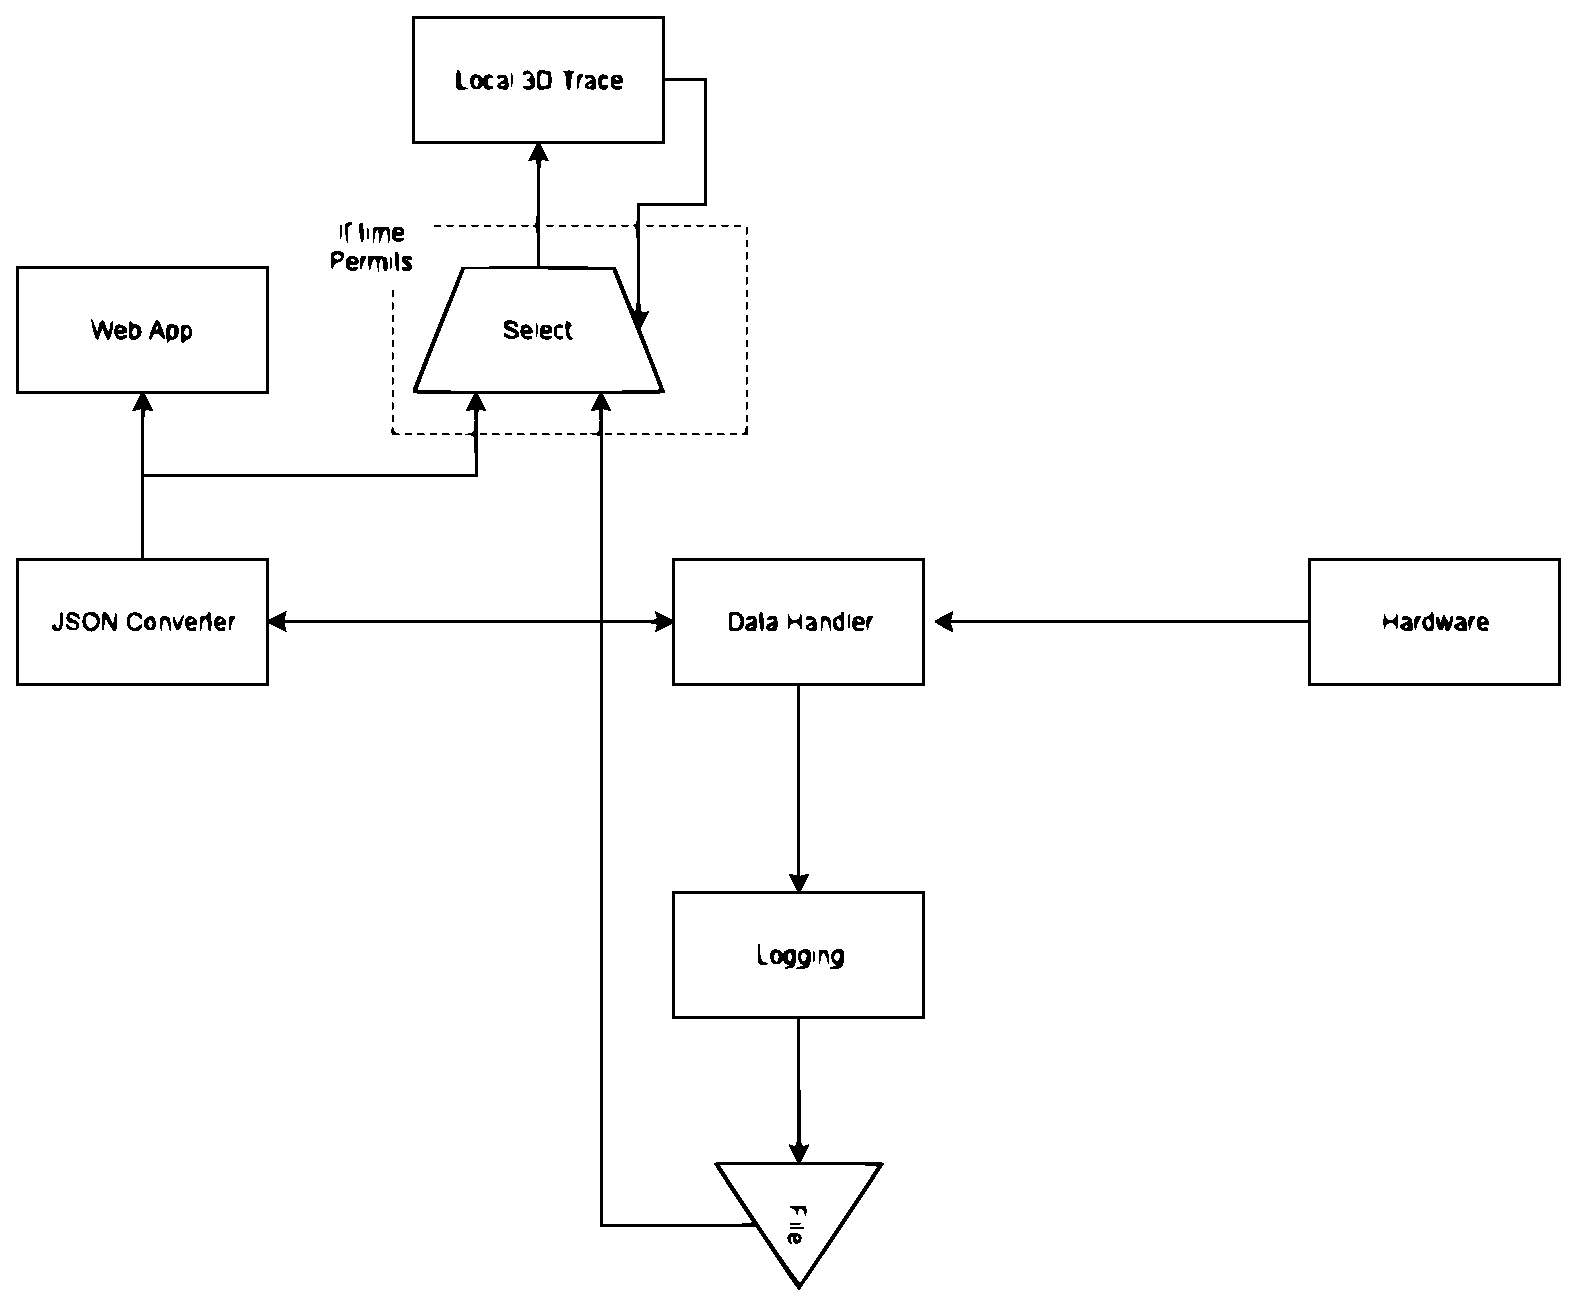
\includegraphics[height=8cm]{datahandel}
        \caption{A high level view of the Data Handling system and its interactions}
        \label{fig:handel}
%    \end{subfigure}
\end{figure}



\subsection {Logging}
Author: Glenn Upthagrove \\
%\subsubsection {Design}
The logging portion of this project shall sit inside the data handling module. The data handling module shall be the interaction with the hardware that collects the data from the hardware after receiving it from the antenna. The logging shall be a fairly simple component. Once the data is collected from hardware by a C module, the data will be converted into a JSON format by a Python module. Once the conversion is completed the data will be passed to alter portions of the pipeline, but also into the logging component. The component shall take in this data as a string. The module will then open a new .dat or .txt file if it is the first piece of data, if not, it will have the correct file already open. After this the data will be appended to the file. This will loop back up to the beginning and it will wait for the next piece of data. The logging component shall actually be its own process, communication with its parent, the data handling process, through a pipe. This is done because it gives timing for free. The logging process will write one data point, and then loop back to the top of its standard operations and wait for a new incoming piece of data, but instead of implementing any sort of complicated timing mechanism to wait for the next data point, it will simply hang until the pipe is filled with data again, which is given for free by the existing implementation of pipes. This allows the logging process to be kept simple, straightforward, and stable. \cite{refjson} \cite{refpython} 
%\subsubsection {Testing}
This module shall have several unit tests, which can be easily done by faking good and bad data. A fake parent process that creates fake data can be easily created to pass fake data in through the same pipe that will be used with the actual data handling module. This could be easily extended to random testing with a loop and random data generated by the fake parent. The random testing portion will pose a few extra challenges, as making fake bad data at random is simple, but creating good data is slightly harder. In mathematical terms, the set containing bad values has a far greater cardinality than that of the set of good data values. 
%\subsubsection {Tools}
The logging module shall be completed before the Data handling module. This will allow easier integration into the data handling module later, as the binary will already be compiled and tested before hand, and can be included in the new process spawning section immediately. This will allow the testing of the data handling module as a whole to be available at the same time as unit tests, immediately after completion. This section draws heavily from lessons learned in operating systems I and both software engineering classes. The file I/O for C that was taught in operating systems I is the fundamental knowledge required to create this module. The interaction between this module and its parent is also covered in this course, as it teaches process spawning and pipes. The testing required for this module are all covered in the second software engineering course, and those tools, specifically unit tests, shall be heavily implemented here.  
\subsection {Local 3D Trace}
Author: Glenn Upthagrove \\
%\subsubsection {Design}
The 3D trace will be a standalone system, created utiliziing OpenGL, which is an Application Programming Interface (API). The API shall be accessed through the a program written in the C++ language. The C++ language is fast, but also object oriented, allowing for abstraction and encapsulation of dome of the more complicated functions of the system. The program itself shall read in data from a file, which is in a JSON format, and then translate that data into vertices, each one representing the position of the rocket in one second intervals. The vertices shall be connected with a GL\_LINE\_STRIP topology. The ground shall be represented by a GL\_QUAD\_STRIP, making a large square plane, which shall then have a texture mapped to it of the area at which the launch is occurring. There shall be a preliminary module which reads in the file, converts it to a string, and then uses the string tokenizer function (strtok), to break it apart based off of the keys in the key value pairs for the JSON formatted flight data. This data shall be passed to a second module that converts the data into vertices, and connects them as a line strip, then stores this into a either a display list, or a vertex buffer object, depending on if the data was sufficiently large to justify the later. The third module would create a sufficiently large plane for representing the ground, reads in a .bmp file, converts it to a texture, and then maps the texture to the plane. The final step would be final display. Several libraries shall be utilized by this module, the OpenGL extension wrangler library (GLEW), and the OpenGL utility kit (glut). \cite{refopengl} \cite{refjson} 
%\subsubsection {Modes}
If time permits, a second mode will also be implemented, allowing data to come in through STDIN and be converted one vertex at a time, and update the trace in near real time, allowing for the tracking of the rocket in 3D during the flight. Also if time permits a sky box with a generic sky image could also be added, as well as the use of a vertex shader to transform the plane representing the ground based off of real topology data. Another addition would be the addition of and idealized model projected forwards based off of tall the data it had collected up until that point. Some of the tools used for the OpenGL programming will be tools provided by Professor Bailey of Oregon State University, which are being used with his express permission. 
%\subsubsection {Testing}
This system can be made at any time relative to the other modules, as it is a standalone system. It however would be preferable to finish the data handling system prior to the creation of this system, as the expansion of this with a near real time mode would be made far simpler if the system earlier in the pipeline that would send that data was already operational. Testing for this shall be done with a fake data creation process, which will create data using simple kinematic equations, and write them to a file for the 3D trace to then read and present. The file reading component can be tested individually with this file to see if the data read in matches. The vertex conversion component can be tested by logging all the data it is converting as it makes the vertices. The display portion can be tested by visual inspection when run, after the previous modules are proven to work sufficiently well. 
%\subsubsection {Tools} 
This creation of this system shall require th skills learned from computer graphics, as well as the introduction to computer science courses. The use of OpenGL as an API and correct manner in which to implement specific graphical elements come directly from the course work of introduction to computer graphics. The interaction of this API in C++, as well as the creation of a solid underlying system for handling the data comes from the C++ learned in the introductory courses. Data structures also lends a hand in the data handling first module, and the file I/O in that same module comes directly from Operating Systems I. 
An overview of design can be seen in Figure 2, where the left represents the near real time mode, and the right represents the post flight mode. 
\begin{figure}[h]
    \centering
%    \begin{subfigure}[Figure 1a]{0.3\textwidth}
        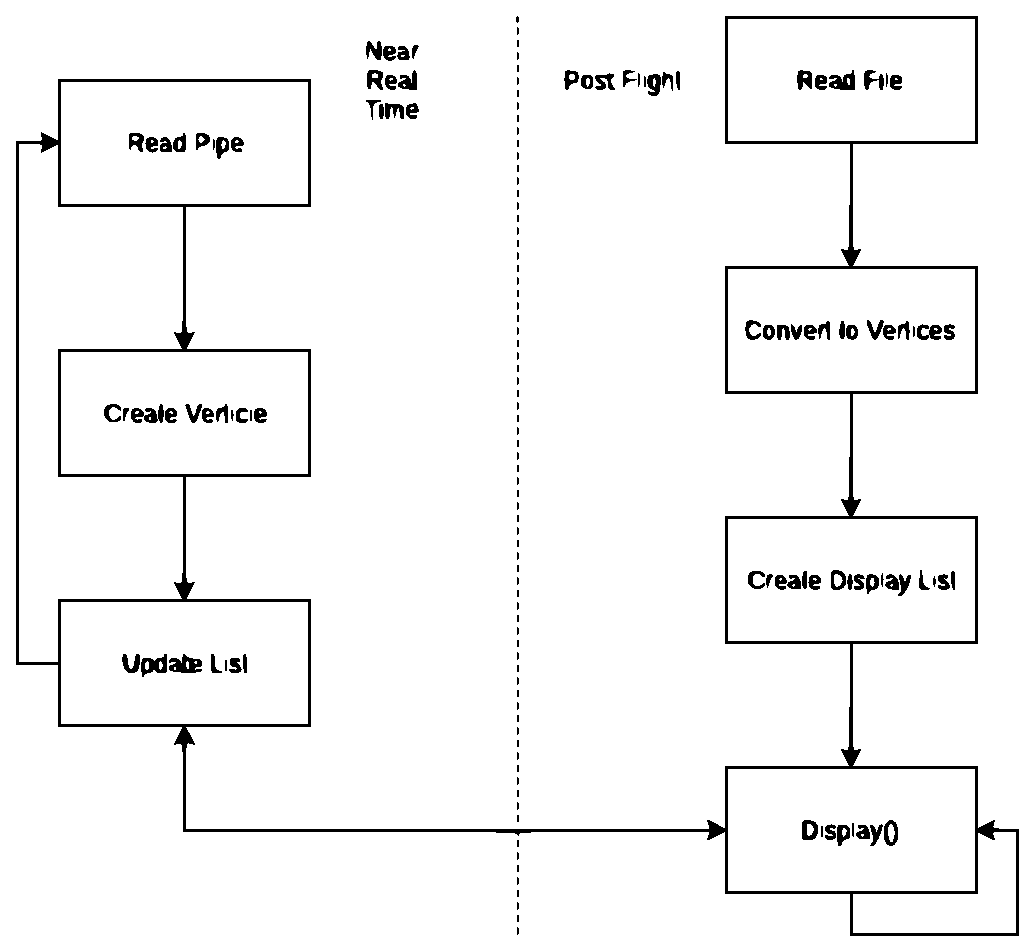
\includegraphics[height=8cm]{3DTrace}
        \caption{A high level view of the 3D Trace with both modes described}
        \label{fig:handel}
%    \end{subfigure}
\end{figure}
\subsection {Visualization}
Author: Sam Hudson\\
The open source JavaScript framework D3 will be used for rendering visualizations based on telemetry data received from the rocket. D3 is the best tool for creating these visualizations because it will allow for tight integration between data points making the visualizations more realistic. There will be three key visualizations. A speedometer for tracking the speed of the rocket throughout its flight, an altitude tracker used to track the rocket’s altitude in respect to the earth’s surface and a trajectory plotter which will plot an estimate of the trajectory based on existing telemetry data. The data used to render these visualizations will be in the form of a JSON object which will contain altitude, gps, velocity and timestamp data. Each visualization will be listening for new data added to the database (MongoDB) attached to the web application. This means that data visualizations can be updated in real time improving tracking and monitoring accuracy. All three visualizations will be displayed on the homepage of the web application to make for easy access. The speedometer visualization widget will utilize velocity data from each JSON object to represent the speed of the rocket throughout its flight. The speedometer will have two rates to represent speed; both mach and miles per hour. The altitude visualization widget will use the altitude data from each JSON object to position a 3D rocket object in a 3D space representing earth's surface and different layers of the earth’s atmosphere. This will give engineers tracking the rocket a better perspective of the rockets altitude in respect to the earth's surface. The altitude visualization will support zoom functionality which will allow users to pan further out relieving more layers or pan in to see the rocket in respect to a specific layer. A ruler will be positioned on the side of widget listing both miles and feet. The trajectory plotter visualization widget will be used to track the rockets position in real-time and also estimate its future position. This widget will make use of all elements of the data objects including, altitude, velocity, gps and time. The trajectory plotter visualization will contain a 3D globe object and a 3D rocket object. The rocket object in respect to the earth object is positioned based on the telemetry data stream. A trail will be also generated based on the rocket’s velocity. The trail will be color coded to indicate the level of acceleration at a given time. The colors will be categorized as follows: red indicates slower than existing average, yellow indicates inline with average and green indicates faster than average. Creating multiple listeners will allow for multiple asynchronous data streams. The listeners attached to each widget will receive data in an asynchronous fashion meaning data will be synchronized with the web page without requiring the page to be refreshed or interrupting the interactive experience. Each widget will be defined in separate JavaScript files to enhance maintainability. Using visualization tools to effectively track the rocket is a critical requirement to ensure the success of the mission. 
\subsection {Front-end}
Author: Sam Hudson\\
The front-end web framework Materialize will be used to design the web application. Materialize is a responsive frontend framework which will enhance user interactive experience and improve the overall interface design. Providing an intuitive and responsive user interface will make it trival for engineers to view important information about the rocket’s flight. The web application will be separated into five pages a main page, a page featuring the speedometer visualization, a page featuring the altitude visualization, a page featuring the trajectory plotter visualization and a page explaining more about the visualizations and how they work. The main page will contain a dashboard featuring all three visualizations widgets organized into three columns of width four. All pages will contain a navigation bar which features the AIAA logo, navigation elements and the current date and time. In addition all pages will feature a footer that will list copyright information and other additional information related to the organization. Splitting reusable code into separate files such as the navigation and footer makes maintaining the project a lot simpler. For example a changing the value of a HREF tag in an anchor element placed in the navigation would only require one update vs having to update each element on every page. This is a dynamic design technique which speeds up the development process. The materialize icon set will be used throughout the web application to improve usability. One benefit of using Materialize as a front-end framework is that it’s fully responsive. As the launch site will be remote it may be inconvenient to take larger devices. Adding adaptability for mobile web clients is essential. Materialize is very useful in that capacity by providing media CSS sets specific to different screen sizes. This works nicely in conjunction with D3. All graphics rendered by D3 are scalable vectors that respond well to changes in screen size. Another benefit of using Materialize as a frontend framework are the many built in mobile components. For example when the screen size becomes lower than a specific size, which can be defined at the discretion of the developer, an icon appears which reveals a collapsible mobile menu. In addition to rendered graphics on each visualization page there will also be tables listing different data values that are used in each data visualization. For instance, the altitude visualization page will have two columns for altitude and time. These tables will live under visualization widgets. To improve the efficiency of the web application both CSS and JS will be minified. The minification of CSS and JS will improve page loading time and reduce the total size of the project. Materialize makes it easy to integrate style changes. Common changes such as theme colors can be defined for all elements pretty simply in the main materialize CSS file. Materialize provides a lot of components that can be utilized. One useful component to have when loading content on a page is a preloader. Materialize had many determinate and indeterminate preloaders which can be useful to show the user that content is rendering. 
\subsection {Server-side}
Author: Sam Hudson \\
The server-side framework Flask-PyMongo will be used build the web application and API. Flask is a lightweight server side framework and PyMongo is a tool used for interacting the MongoDB. PyMongo is required because Flask doesn’t natively support Object Relational Models. As mentioned in the front-end development section the web application will consist of 5 pages. These five pages will contain widgets that rely on data contained within MongoDB. The main backend application will have 5 different routes: “main”, “altitude”, “speedometer”, “trajectory” and “about” these endpoints will be managed by handler functions that will be responsible for managing interactions with each page. Jinja2 is the templating engine that will be used to render each page. There will be three templates in total. One that will define the main page for the dashboard, one that will define the layout for the visualization pages and one that will define the about us page. Each handler function will gather related data for that specific page and pass that data into the jinja2 page rendering function. Data that’s specific to each page includes the page title, table contents, visualization widget data and current navigation information. An application programming interface will also need to be defined for access to data store in MongoDB. Two additional handler function will need to be defined for getting and setting telemetry data. The object model telemetry\_package will be defined with attributes: altitude, gps, velocity and timestamp. Making a get request to the telemetry\_package endpoint will return a list of all telemetry packages for use in D3 visualizations whereas the post endpoint will be responsible for adding telemetry packages to the database. Each call to the rest API will require a secure token which will be verified on the server. A function will be defined to authenticate and authorize selected transactions. This is an important security feature because it’s important to verify the sender is who they say there are. Authenticity can be validated because only systems with access to a secret token will be able to authenticate against the API. D3 visualizations will be defined in JavaScript and only interface with the API. Telemetry data will not be served through standard page handlers. Flask has a built in local development server which will suitable for hosting this web application and API. Only localized access is required the application will not be public facing. MongoDB is the best database technology for the specific case. Telemetry data will be stored as JSON objects. JSON Objects are the format in which MongoDB stores data within its database. This means little effort is required to store this data because data sent to the API will already be in the correct format to store within the database. MongoDB is a non-relational database that scales very well and can store large amounts of data. MongoDB is a high performance database technology that can handle many different requests.
\subsection {Connection Overview} 
The basic topology of the system in its entirety is a pipeline. At the beginning raw data comes in from the sensors, and at the other end is displayed in a meaningful way to the screen. There are of course a few pieces that do not fit perfectly into the pipeline model, the logging module and the local 3D trace for instance, but the main goal, and the modules meant to achieve it, fall fairly neatly into this topology. The first few stages are done on the rocket, where the data is collected, sent to a Kalman filter, packaged neatly and transmitted. These modules shall primarily be authored by Michael Elliott. The middle stage is where data is received by hardware on the ground station, collected from hardware, and converted to JSON. These modules shall primarily be authored by Glenn Upthagrove. The final stage, the visualization, receives the JSON data, goes through the web API, into a mango DB module, into the web application, and finally to the display. These components shall primarily be authored by Samuel Hudson. The logging module, the log file, and local 3D trace shall sit next to the main pipeline. The overview of the abstracted pipeline is illustrated in Figure 3. 
\begin{figure}[h]
    \centering
%    \begin{subfigure}[Figure 1a]{0.3\textwidth}
        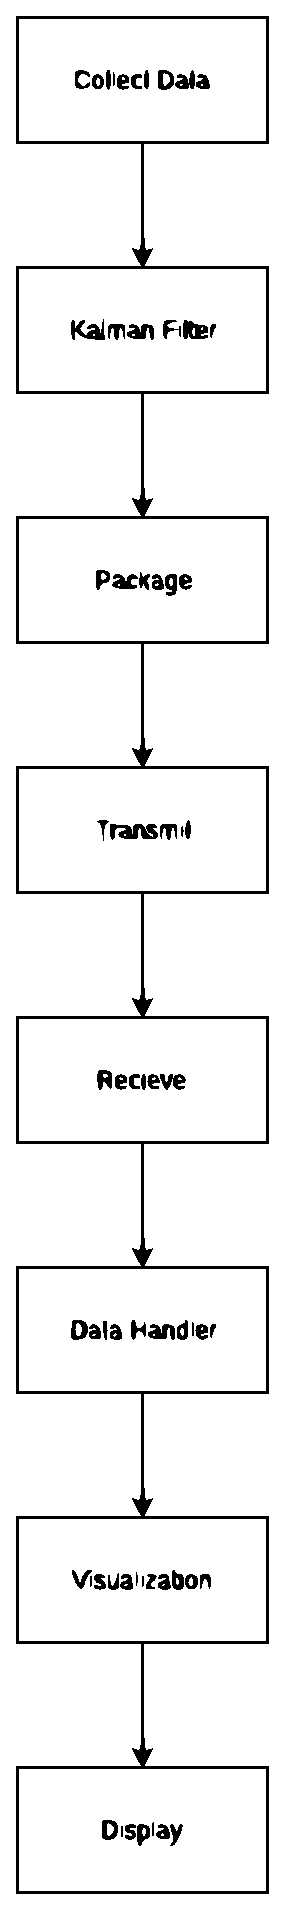
\includegraphics[height=12cm]{basicpipeline}
        \caption{An abstracted view of the software pipeline}
        \label{fig:handel}
%    \end{subfigure}
\end{figure}
\subsection {Conclusion}
All of these components will fit together into the final collection of
software used to track the rocket during flight.
This will help achieve the goal of reaching 100,000 feet of altitude.
Each component is an important cog in the overall machine, and they
all must fit together properly in order for us to succeed.
This is why having a well thought out design is so important for our project.
It ensures that all of the important pieces fit together well and
gives us a road map for our testing in the future.
With such a critical mission, there is very little tolerance for
error, so testing thoroughly and designing properly is paramount.

\section{Technology Review For Micahel Elliott}
\subsection{Abstract}
In this project we will design and build recovery and telemetry systems for a rocket that will reach a target altitude of 100,000 feet.
We will create telemetry interfaces for tramsmitting and receiving data and avionics for the recovery of the rocket.
This problem statement document will cover the details of the challenge, the outline of the proposed solution, and metrics to judge the success of the project.
The main challenge will be to design a means of collecting, interpreting, and transmitting data on the rocket, in addition to receiving, interpreting, and displaying data on the ground.
Additionally, we will be working with embedded hardware, the constraints of which we will have to work within.
Our project will be successful if we can collect, transmit, and properly utilize the flight data, both in flight and to recover the rocket.
For this project I have been designated by the client as the main contact with the group.
My main focus is the code running on the rocket itself.
I will be working closely with the electrical team that is designing the hardware.
\subsection{Data Noise Filters}
One of the problems we will encounter in sending a rocket 100,000 feet in the air is the collection and interpretation of accurate data from the sensors.
At such high speeds and low pressure, there will be a lot of noise in the data.
We will need to collect and utilize the data we receive from the sensors even though it may be inaccurate.
This means that we need a way to remove the noise from the readings.
The following are a few options we have considered to help remove noise from the data.

\subsubsection{Antonyan Vardan Transform}
An Antonyan Vardan Transform is an algorithm that helps remove noise from data.
There are many ways to filter noise from data, and an Antonyan Vardan Transform strikes a great balance between simplicity and effectiveness.
An Antonyan Vardan Transform takes multiple averages of the data set provided and uses the standard deviation to remove outliers.
The first step is to retreive a predetermined number of samples.
This is the period of the transform.
After the set number of samples is collected, the average of all of the samples in that period is taken.
Now all data points more than one standard deviation from the mean are removed from the set of samples.
At this point all of the data is averaged again; this is the final value.
The Antonyan Vardan Transform is then performed again after every n samples where n is the period.
This algorithm is very simple to implement, and it is effective at ignoring outliers in the data.
This method is also not quite as effective as one needs on a rocket, since the noise is sometimes of a greater magnitude than the data itself and because the data needs to be accurate down to a small time increment and the Antonyan Vardan Transform is more effective with a larger period.

\subsubsection{State Observer}
A state observer is an algorithm that combines and cross references the data from a selection of inputs in order to create a known state that is tracked internally.
With this method we can, for example, take the altitude data from a GPS and the atmospheric pressure data from a barometer and cross reference them to get a more accurate final altitude value.
This is especially useful because different sensors will behave differently under different conditions, so we can rely more on one or the other depending on the readings.
This method is also relatively simple to implement, which is important in ensuring the correctness of safety critical code.
There are different variations of state observers as well, for example one can have multiple layers of observers that each input into the other to cross reference data incrementally.
Or one can have two observers, one that estimates high and one that estimates low.
This way the actual state is always in between the two.
Additionally, to make an observer more effective one can even perform an Antonyan Vardan Transform on the data going into the observer.
Observers have a few limitations.
Firstly, there is relatively little actual filtering of the data beyond the cross referencing of the inputs, so if the inputs are extremely noisy, the internal state will be inaccurate.
Also they don't account for the changing state of the sensors themselves, just the environment that the sensors are receiving input from.
This can present a problem in dynamic applications.

\subsubsection{Kalman Filter}
A Kalman filter is an algorithm that uses linear quadratic estimation to filter out statistical noise.
A Kalman filter uses a model to make predictions for the future state, and adjusts those predictions based on input.
It begins with a known state, and compares each new input value to the ideal predicted value.
It weights the predictions and the inputs to reach a reasonable middle ground based on how much noise there is expected to be in the inputs.
The predictions are made based entirely on the current state and the internal model for the behaviour.
This means that a Kalman filter can be run in real time.
It also means that it can be run on limited resources provided the state and model are not overcomplicated.
We chose a Kalman filter as our method of removing noise from the readings because of the additional capabilities it gives us over the other options.

\subsection{Communication Protocols}
Another problem we will encounter while travelling at high velocity over 20 miles in the air is potential issues with radio communication.
The atmosphere will be thin, and there may be RF interference.
Even at such high speeds and long distances with a less than ideal transmission medium, we still have to ensure ensure that the data received by the ground station from the rocket is uncorrupted and that it is received in the correct order.
In thinner atmosphere and at speeds over Mach 1, especially with potential interference from the body of the rocket itself, there is potential for high packet loss.
This is why we need to make sure our transmission protocol is robust and efficient.

\subsubsection{TCP}
TCP is the standard protocol for connecting between two computers over the network.
TCP fulfills our requirements because it ensures the ordering of packets, performs error checking, and makes sure that every packet arrives to the receiver.
With TCP we do not have to worry as much about reliability because TCP will handle all of the error checking for us.
The TCP protocol works by ordering the packets and then keeping track of which packets have been received.
Once the receiver gets a packet, it acknowledges the receipt of the packet to the sender.
This way the sender knows not to send the packet again.
If the sender receives no acknowledgement for a packet it sent, it will send it again.
If the receiver receives a packet that is ahead in the order of the packet it is expecting, it will request the missing packet from the sender.
This way both the sender and receiver know what has been sent and received by the other.
A TCP packet containing the minimum amount of data required to send to the ground station would be about 40 bytes long.
Depending on the bandwidth of the radio this may or may not be an appropriate size.
Also there are already library implementations for TCP, so development time would be relatively short.
The main issue with TCP is that with the potential for such high packet loss, it would be a waste of precious computing resources on the rocket to keep sending the same dropped packets over and over again.
This is especially concerning because if the outbound transmission buffer on the rocket fills, the new packets will be dropped or the packet creation will be stalled, neither of which is appealing especially because the packet buffer has the potential to be very small, perhaps even smaller than 40 bytes.
While it would be nice to acknowledge the receipt of every packet, it does not seem feasible to continue down that path.
We will likely have better luck dealing with dropped packets.

\subsubsection{UDP}
Unlike other protocols like TCP or SCTP, UDP does no error correction and does not require an established connection to begin sending data.
This means there is no protection against dropped packets, reordered packets, or duplicates.
UDP is a very low overhead protocol and leaves most of the data handling up to the user.
This protocol would be preferable to TCP because with the limited processing power and relative time sensitivity of the data, it is preferable to drop a packet than to retransmit.
Also UDP does not require any response from the receiver, meaning the rocket can focus its processing power on other more important tasks.
UDP does contain a checksum of the data to ensure that there is no corruption within the packet.
A UDP packet containing the minimum amount of data required to send to the ground station would be about 28 bytes long.
Depending on the bandwidth of the radio this may or may not be an appropriate size.
Also there are already library implementations for TCP, so development time would be relatively short.
UDP seems like a great option compared to TCP for our application.
There are a couple potential downsides to using UDP however.
One downside is that the rocket will have to spend CPU time computing the checksum of the data.
This would normally be a good thing because it ensures that the packet is not corrupted, but it takes precious CPU from the other critical tasks on the rocket.
Another issue is that 28 bytes per packet may still be on the big side especially if the transmission buffer is small.
These potential issues with an otherwise great looking protocol are why we looked into the next option.

\subsubsection{Custom}
With a homegrown protocol, we can make it however we like.
The main downside to using a homegrown protocol compared to something like TCP or UDP is that the development time will be significantly longer.
But using a custom protocol will give us much more control over the data and will allow us to streamline the connection as much as possible.
The streamlining of the connection is of the utmost importance due to the limited computing resources on the rocket.
We plan on basing our custom protocol on UDP but with a few key changes to improve it.
First we'd like to cut down our packet size to about 20 bytes.
This would allow us to transmit in as few clock cycles as possible with a lower bandwidth radio.
Also since we will already be writing code on the receiver to handle dropped packets, we could also write code to handle corrupt packets meaning we could avoid creating the checksum.
Especially if we use a fixed packet structure, all the rocket would have to do is pack the packet and send it, with no other processing on the transmission end.
For these reasons we have decided to go with a custom data transmission protocol.

\subsection{Language \& Tools}
The language and tooling are very important in deciding how to build a system.
Each language has varying levels of speed, safety, and tools available.
For code on a rocket, there is no room for any errors.
Also the code must run quickly on limited hardware.
The language must allow developers to easily write correct code that is also fast.
These criteria quickly ruled out a large number of languages right off the bat.
There were a few languages left over that were obvious choices for the program running on the rocket for a few reasons.
Each of these languages have good support and the tooling required to complete our project.

\subsubsection{Rust}
Rust is a relatively new language and is enticing for a lot of reasons.
One of the main attractions to Rust is the memory safety.
Unlike languages like C, Rust has safety nets in place to prevent memory access errors and other errors of that class.
There are many languages that do this, but Rust does so while still allowing low level control.
Rust is also very fast.
Even though Rust is a new language, it has been extensively tested.
Mozilla is even re-writing the Firefox code in Rust for the speed improvement.
Rust also has lots of libraries for functionality that we may require without wanting to reinvent the wheel.
There are a couple of issues with Rust that would make me hesitate to choose it for our applications.
The main issue is that Rust uses dynamic memory allocation.
This would not be an issue on any system with more than a few megabytes of RAM, but our rocket is going to have such limited resources that this will present a problem.
The problem is that Rust reclaims memory through reference counting rather than garbage collection.
This means that there is the potential for memory fragmentation to occur.
For a system with such critical code there is no room for error when it comes to memory allocation.
Unfortunately this issue will likely knock Rust out of the race.

\subsubsection{Ada}
Ada is an old language that has been used very frequently in critical code.
Ada is one of the most commonly used languages for projects done by the Department of Defense due to its maintainability and safety features.
Ada was also used on projects like the Cassini probe.
Ada has a lot of built in runtime checks and compile time checks that prevent code from compiling if it doesn't adhere to the strict user defined rules.
All these checks make Ada a really attractive language for safety critical code.
Additionally, Ada is very fast.
It will play nicely with the limited resources on the rocket.
One downside to Ada is that the development time is generally longer than for other languages because it is so verbose.
Also adding to the development time would be familiarizing ourselves with the language.
While I am at least familiar with the structure of the language due to my research, my team mates are not and neither are the members of the ECE team who will also need to be able to read our code.
I would personally love to use Ada for our project, but the increased development time required makes it impractical to use within our given timeframe.

\subsubsection{C}
C is the golden standard for programming languages.
It has been around for as long as Ada and Fortran, and is as popular as JavaScript.
C provides no safety nets which means it is very fast, but it is also difficult to write safety critical code in C.
This is why if we use C we plan to use strict programming guidelines and perform static analysis on our code.
If we follow strict guidelines and test our code appropriately, there is no reason why it can't be as safe as Ada.
The reason C code is sometimes bug ridden is because the programmers test poorly and use poor programming practices.
Especially with the large number of language tools like static analyzers, programming critical code in C is easier than ever.
Static analyzers examine the structure of the code and point out potentially problematic structures in the code.
If we roll all of this together with the familiarity of C to the ECE team who will have to read our code, C seems like a great option provided we take the proper precautions.

\section{Technology Review For Samuel Hudson}
\subsection{Abstract}
This document will review technologies that will be considered for use in the design and execution of our final product.
\subsection{Visualization}
\subsubsection{Introduction}
During the deployment, in-flight and descent stages we will be tracking the rocket through radio telemetry. This data will be sent from a transmitter attached to the rocket down to the ground station. When the data is received by the ground station the data will then need to be organized and displayed to all parties following the launch. We will be designing a web application that imports telemetry data and renders useful information graphically such as trajectory, altitude and velocity. There are many frontend libraries for representing data graphically. Listed below are three contenders for providing this functionality. 
\subsubsection{D3.js - Data Driven Documents}
D3 is a robust open source JavaScript library for rendering visualizations and data interaction. D3 supports a wide range of different visualizations that are not available with standard charting frameworks. For instance, D3 supports 3D object generation, this will be useful when superimposing a rocket vector on a globe for visual tracking. D3 has the capacity to render visualizations with vast amounts of data making this tool scalable. We will be gathering large amounts of data during the tracking process and a tool that can support in this capacity is essential. Another great benefit of D3 is the level of interactivity supported with visualizations. Visualizations are rendered as scalable vector graphics meaning each component of the visualizations is manipulable at the discretion of the developer. Although D3 is feature rich tool for rendering visualizations and data interaction the implementation from a programmatic standpoint is complex versus other visualization libraries. Using D3 will enhance the interactivity  of the web application at the cost of taking longer to implement. 
\subsubsection{Chart.js}
Chart JS is an open source, minimalistic JavaScript chart library. Chart JS provides 8 chart types for visualizing data these include line, bar, radar, pie, polar, bubble, scattered and area. Chart JS was designed with simplicity in mind with clear documentation and an easy to use programming interface. Although Chart JS is easy to use it only offers basic visualizations and does not scale when introduced to mass amounts of data. Another limiting factor of Chart JS is interactivity. Chart JS does not support any data interaction. Chart JS takes advantage of the canvas element in HTML5 to render visualizations meaning that a single html element is rendered therefore data points cannot be modified. Defining a simplistic visualization in Chart JS requires less code than most visualization frameworks. Using D3 will enhance the functionality of the web application at the cost of taking longer to implement. 
\subsubsection{C3.js}
C3 is an open source, minimalistic JavaScript chart library that is based on the D3 library. C3 uses same approach for rendering as D3 but with a focus on charting. Meaning C3 supports data interactions as charts are rendered as scalable vector graphics where data points are manipulable. C3 requires less code to define charts and supports features such as tooltips, legends, gridlines and customizable tick labels. As C3 is specifically designed for chart render features such as 3D object rendering are not supported. Using C3 will simplify the implementation process and scale well with large datasets but does not provide the extra visualization that will be useful when rendering 3D objects. 
\subsubsection{Conclusion}
The most encompassing tool for rendering charts and visualizations is D3. D3 will enhance the interactivity of the our web application and improve the representation of our data. Although, as mentioned, the downside of using D3 is the complexity of the interface the benefit of better visualizations vetoes other visualization library use. Other libraries such as C3 and Chart JS will simplify the implementation process but does not provide the extra visualization that will be useful when rendering 3D objects to show the rockets positioning in respect to the surface. 

\subsection{Front-end Web Frameworks}
\subsubsection{Introduction}
The most effective way to speed up the development process of the frontend is to use a framework. The framework will provide a basic structure making construction more convenient. Listed below are three different frontend frameworks and their respective advantages and limitations. 
\subsubsection{Materialize}
Materialize is an open source front-end framework built by Google. Materialize provides features such as inline animation definitions, flow text, chips and cards. Similar to the other popular front-end framework bootstrap, materialize supports a grid system, icon sets and responsive elements. From an aesthetic standpoint Materialize is more modern in appearance and provides a richer set of animations enhancing the overall user experience. Materialize is a new front-end technology and still requires some greater refinement in its grid system. The grid system is limited in the number of intervals it supports. Using Materialize will improve the frontend development process and provide a greater experience for users of the web application because of integrated animated feedback when using components and a modern look and feel. 
\subsubsection{Bootstrap}
Bootstrap is an open source front-end framework built by Twitter and has been greatly contributed to since then. Bootstrap is well supported and has responsive features ideal for users who access web applications via a mobile browser. Bootstrap is more robust than Materialize and has been around for a longer time. Bootstrap has an extensive list of components which makes element construction simpler. Bootstrap is extensive in terms of lines of code can become difficult to contribute to and modify. Using bootstrap will improve accessibility of our web application because of the responsiveness in mobile environments but provides a lot more than what is needed which could hinder application performance and development speed. In addition Bootstrap can be difficult to contribute to as JavaScript is forced to Jquery and styles convolutedly defined. 
\subsubsection{Semantic-UI}
Semantic UI is an open source front-end framework. Semantic UI provides a set of customizable UI components that have support many different unique themes such as Chubby, GitHub, and Material. Themes in Semantic UI make styling much simpler and can speed up the development process. Although Semantic UI has a large amount of customizable features and provides a better interface for style integrations, similarly to Bootstrap, Semantic UI is extensive in terms of lines of code can become difficult to contribute to and modify. Using Semantic UI will make customizability a lot simpler but this benefit does not outweigh the bulk of additional features that will not be used and hinder the performance of the application.
\subsubsection{Conclusion}
The best front-end framework for designing the interface for the rocket reporting web application is Materialize. Although Materialize is a new front-end framework and could do with additional development on the responsive grid system it is has more aesthetically pleasing components and nice features such as integrated animated feedback. Materialize is lightweight and also an easier framework to add custom style integrations.
\subsection{Server-side Web Frameworks}
\subsubsection{Introduction}
In order to bridge communication between the server and web client an interface has to be designed to handle routing, database interaction and web page rendering. During the rocket launch telemetry data will be gathered, converted to JSON and stored in a database. A server side interface will be responsible for interacting with such data and serving to the web client for presentation. A server-side web framework would speed up the design process and provide features as mentioned out of the box. Listed below are three different server-side frameworks and their respective advantages and limitations. 

\subsubsection{Flask-PyMongo}
Flask is a microframework for Python that includes a dynamic templating framework called jinja2 which makes rendering content for presentation much simpler. Routing in Flask is also very straightforward and syntactically clear. Another benefit of Flask is that it is a microframework meaning there’s less overhead for the project making the codebase easier to maintain. Flask-PyMongo is Flask and MongoDB combined for ORM(Object Relational Mapping) support this allows for the configuration of relational models. This is an important feature because the web application will be required to interact with a database storing JSON objects and an easier way to model data objects will speed up the development process significantly. Though Flask is simplistic in nature and easy to use it lacks in support and documentation and requires the importation of many other modules to provide greater functionality. Using Flask will simplify the implementation process and provide a simplistic interface between the client and server. Although Flask requires the additional modules such as PyMongo to support ORM.
\subsubsection{Django}
Django is an all encompassing Python web framework. Django provides a lot of features such as routing, ORM, authentication and template rendering. This makes it much easier to bootstrap the development process. Django is well supported and has a larger contribution base. Although Django is a powerful web framework with a lot of features it is less suited towards this application where the requirements are more simplistic. Using Django as a server-side framework would help speed up the development process but provides unnecessary features which are outside the bounds of this project.  
\subsubsection{Express JS}
Express is a flexible web framework designed integrate seamlessly with the javascript runtime environment node js. Express provides a good for lightweight applications and has a thin layer of web application abstracting away a lot of complexities in presentation and business logic. As Express JS is written in JavaScript this will create a consistent language between the backend and frontend. Express supports ORM through the importation of Sequelize, like flask this a module that has to be imported in order to add additional functionality. Using Express JS would create consistency between the backend and frontend in addition Express JS is a lightweight framework that provides the bare minimum to get the job done, although it still requires the importation of additional modules and a slight learning curve.
\subsection{Conclusion}
Flask is best backend framework for the job. Flask makes routing and templating extremely simple. Although additional modules such as MongoDB will have to be imported to create ORM functionality, for this specific project Flask is best Server-side framework. Using Flask will simplify the implementation process and provide a simplistic interface between the client and server.

\section{Technology Review For Glenn Upthagrove}
\subsection{Abstract}
In this technology review various solutions are explored and compared to solve three sections of the 100k Rocketry project for the computer science sub-team. The first explored is three solutions for making a 3D trace of the flight path. The second is how to log the data coming in from the hardware on the ground station. The final piece is an exploration of how to handle the data coming infrom the hardware before it is passed off to logging.
\subsection{Role in Project}
For the most part, I shall be focused on software running on the ground station. The data shall be travelling through a pipeline, starting at collection on the rocket, and ending at visualization. I sit mostly in the middle, where the data is collected from the hardware, formatted, logged and passed further down the pipeline. I also will handle a small protion of the visualization, as I shall be doing the 3D trace program. 
\subsection{Overview of Project}
In this project we are, at a high level, trying to track a rocket during its flight. This implies that our job is more specifically, to clean up the data of noise before transmission from the rocket, to gather the data as it comes in from hardware on the groundstation, handle and format the data, log it, and display it in a meaningful way. The sections covered in this document are the handling of the data, the logging of the data, and the 3D aspect of the visualization. 
\subsection{3D Trace}
This section covers possible solutions for the 3D trace of the flight path. Author: Glenn Upthagrove. 
\subsubsection{Criteria} 
The tools used to make the 3D trace must meet certain criteria. The first being that it must be capable of running on as reduced a hardware profile as would be seen on a Raspberry Pi, as it is very possible that will make our ground station. It must be capable of running on many different graphics accelerators, not specifically to any on emanufacturer. The final criteria is that it must be easy easy enough to program in, sych that it is reasonable to complete in the reduced time window alloted to our group. 
\subsubsection{OpenGL}
The OpenGL Application Programming Interface (API) is a simple high level abstraction of graphics card interaction controlled by the Khronos group \cite{refopengl}. This allows the programmer to leverage the Graphics Processing Unit (GPU) is rendering 3D scenes. The API is simple, and allows significant results in a much shorter time frame than other graphics libraries. It is also a cross-platform solution, allowing implementation on many devices, such as the Nvidia Jetson TK1 or most desktops \cite{refopengl} \cite{refjetson}. It is also the most widely used graphics API in industry, giving us access to a robust development community \cite{refopengl}. The library can also be accessed through most programming languages \cite{refopengl}. There are faster options on the market, such as Vulkan, but are usually much harder and more specialized than OpenGL\cite{refvulkan}. This library also has bonuses in personal familiarity and simplicity, making implementation time much shorter, and eliminating most if not all time to learn the required materials for the trace. This is an important consideration since our full software suit must be working by the end of winter term, in time for the practice launch. 
\subsubsection{WebGL}
WebGL, also of the Khronos group, is an API for using the reduced form of OpenGL, known as OpenGL ES, on the web, through ECMAScript and the HTML5 canvas element \cite{refwebgl}. This API allows for a more basic 3D experience, but capable of being run on less powerful hardware. The requirements of the 3D trace of the flight path are such that these reduced capabilities should cause no degradation in quality. This library also should work well on a Raspberry Pi, if that so happens to become the ground station, as it is supported by web browsers that Linux can run, such as Firefox and Chrome, and the underlying OpenGL ES is supported by the Raspberri Pi \cite{refwebgl} \cite{refpi}. WebGL also has the added bonus of being very similar to OpenGL, making crossover fairly straightforward \cite{refwebgl}. 
\subsubsection{Vulkan}
A much younger graphics library under the Khronos group, is Vulkan. Unlike OpenGL it is not a high level abstraction, but instead is meant to be a much lower level interaction layer, that can leverage much more power out of the system, while higher level APIs can stay relatively unchanged \cite{refvulkan}. Vulkan can achieve much of this by clever uses of parallelism in the pipeline \cite{refvulkan}. While this can allow for a noticeable improvement in performance for many graphically intense applications, this would be wasted on such a simple program such as our 3D trace. Vulkan is also much more verbose and requires a much longer development time, especially considering it being very unfamiliar to us. 
\subsubsection{Conclusion}
Considering the requirements of the 3D trace, and the time constraints of our project, I believe OpenGL is the best solution. It is reasonable to believe that due to the reduced hardware profile of a Raspberry Pi, WebGL would be a better solution, however OpenGL is supported on the Raspberry Pi as well \cite{refpiii}. Since the scope of our project is fairly substantial, and we have to be done within one term to meet the date of the test launch, it is more important that we can get all the software completed in time rather than make it as absolutely efficient as possible. Since time is such a limiting factor, the familiarity of OpenGL and the vastly simpler code, makes it a far superior choice for this project than Vulkan. OpenGL is far simpler than Vulkan, more familiar than either Vulkan or WebGL, and more than capable of rendering the trace, OpenGL is the appropriate choice for this project\cite{refgs}. 

\subsection{Logging}
This section covers options for formatting the data for storage in non-volatile memory. Author: Glenn Upthagrove. 
\subsubsection{Criteria} 
The form in which we output the data is critical for parts further down the pipeline. The data must be easily accessable to the pther parts of the system downstream, and thus it is important that it is either stored as it will be used, or at least in such a maner as to minimize reprocessing by later modules. The output should also be human readable, as there shall be an output to a log file. 
\subsubsection{Pipe Delimited}
This would be the simplest way to format and store the data, where each float is separated by a pipe character, and each set of floats is ended by a newline character. This would allow for a very minimalistic formatting process to simply break up the data and write it to a file. The data could be later opened by any of the other portions of our suite for later use. While this is both easy to implement and would minimize processor usage, it would mean that any other program accessing the data may have to do additional formatting to make it useful for that program. 
\subsubsection{JSON}
Java Script Object Notation (JSON) is a widely used format for storing and transmitting data \cite{refjson}. The data can be stored as a variable, written as plain text and then read back into a variable with the same structure. The syntax is familiar to most languages that are derived from C, and thus can be easily manipulated in many of these languages, and most have libraries already available to do this \cite{refjson}. Python has a library readily available to handle JSON, which could be used to make the logging into a file very easy, especially with how well Python handles strings \cite{refpython}. JSON would also make the data more easily available to the 2D visualization, and the 3D trace could be written to use it as well, adding no conversion step in between the log and these two other modules.
\subsubsection{YAML}
YAML (YAML Ain’t Markup Language) is a superset of JSON \cite{refyaml}. It uses very similar syntax, and is in fact more capable, as it can do all the things JSON can do but with extensions on that syntax. It is also similar in size and complexity, but is more human readable, at the expense of parsing ease. When compared to JSON, YAML is less well adapted to our other modules, and unlike JSON, a YAML library for Python would need to be separately installed \cite{refyamlii}.
\subsubsection{Conclusion}
The log shall be stored in JSON. This format is slightly larger and more complex than the pipe delimiter, but also more human readable, and more easily integrates with other portions of the project. JSON is also less readable than YAML, but easier to parse, has more readily available libraries, and will integrate more easily with the rest of the project. These factors make JSON by far the best option. Additional logs could also be easily added in future upon the request of another member of this or any other sub-team\cite{refgs}.

\subsection{Data Handling}
This section shall discuss options for which language or combination thereof to handle incoming packets on the ground station. Author: Glenn Upthagrove.
\subsubsection{Criteria}
The language choice for the module handlign the data once it is recieved by the hardware is critical. this implies that the langauge must forst be able to access the data from the hardware. The language should also consider how easily it can manipulate said data once it is retrieved. The language should also take into account any libraries that are availabel to make these probles easier, such as libraries that can turn data into the chooses output format. Familiarity, while not a deciding factor, should also be factored in, as the time window we have is not broad, and familiarity makes bugs easier to find and fix, which is critical on software that must be running in near real time. 
\subsubsection{C/C++}
The C language is a high level language, but allows one to get very close to hardware, and even drop directly into assembly if need be. C++ is very similar to C, and can for the most part even use C code inside it, but allows for more features, as it is an object oriented language. C and C++ could both be very good options for dealing with the data as it is recovered from hardware, as it allows for very close memory access and manipulation. C and C++ are also very familiar languages to us all, and would reduce the time taken to develop and debug. Storing the data and passing it to other sections would be the downside of C, as it is not as easy to manipulate strings in C as in some other languages.
\subsubsection{Python}
The Python language is a high level scripting language, with similar syntax to C. Python is on average slower at run time than C/C++, as it is not compiled. However Python also is generally somewhat shorter and easier to write than C/C++ and could speed up development time. Python also is often better at string manipulation than C/C++ and could make the passing of data to the rest of the project modules easier. There is also a readily available library for using the JSON format we intend on using in other sections of this program \cite{refpython}. The weak spot however is that Python being generally more abstracted than C/C++ would make the retrieval of the data from the hardware much more difficult to do, on top of running far slower than a C/C++ solution.
\subsubsection{C/C++ and Python}
As seen above both a pure C/C++ solution and a pure Python solution, seem to have certain strengths and weaknesses that correspond quite well. In simpler terms, they complement one another, and the obvious solution is to combine them, which luckily can be done with relative ease. The retrieval of the data from the hardware could be easily done in C/C++, then this solution could either be called by a Python program which takes the data from the C/C++ as a return, or they could be separate modules that are continuously running, and the C/C++ solution passes its data to the Python module over a pipe or through a file. The Python then converts the data to JSON and then passes it along to any other parts of the suite that need the data. The C/C++ portion could also speed up the program more than a pure Python solution.
\subsubsection{Conclusion}
As can be clearly seen from the above discussions, the best solution is the combine the speed and superior hardware access of C/C++ with the better string and JSON handling of Python. Together they can make a very elegant solution for retrieving, formatting, and storing the data as it comes into the ground station. The speed of the ground station hardware will also be superior to the rocket, and thus should have plenty of time to run a simple Python script, especially since part of the work will be offloaded onto a fast C/C++ solution\cite{refgs}.

\section{Blog Posts}
\subsection {Week 1}
\subsubsection{Michael Elliott}
\begin {itemize}
\item \textbf{Plans: }
 This week I plan to get a team together to work on the 100K Spaceport America Demonstration Rocket Project. This is the project that interests me the most and I have already talked to the members of the other teams. The next steps include finding 2 more members for the CS team and talking to Nancy Squires, the project's client, about requesting us as her team.
\item \textbf{Problems: }
  The biggest problem I ran in to during this first week was finding other talented individuals who wanted to work on the project. Many showed interest but did not want to make a commitment.
\item \textbf{Progress: }
  I have found 2 other members for our team and have been in contact with Dr. Squires. Hopefully we will be able to solidify our positions on the team. We also attended the first all team meeting this week since work on the project needs to be started immediately due to the reduced timeline even though we have not been confirmed for the project yet. We used this meeting to introduce ourselves to each other and familiarize ourselves with the project. We also held a second team meeting with all of the avionics teams to start very high level planning.
\end {itemize}
\subsubsection{Sam Hudson}
\begin {itemize}
\item \textbf{Plans: }Discover what is required for CS 461.
\item \textbf{Problems: }Some issues establishing best meeting times for group.
\item \textbf{Progress: }We determined that Monday was the best time to meet with all groups related to the project and Wednesday was the best time to meet for our subteam meeting.
\item \textbf{Summary: }This week I met with the 100k rocket team in Rogers. We discussed project management strategies and I suggested to use a project management tool called Jira. I configured Jira for the team to try. We discussed a few resources to consider for the project including a book discussing aspects of test driven development for embedded C. Towards the end of the meeting I submitted my project preferences. 
\end {itemize}
\subsubsection{Glenn Upthagrove}
\begin {itemize}
 \item \textbf{Plans: }Find projects that interest me. 
 \item \textbf{Problems: }We are having trouble getting in touch with the professor in charge of the AIAA 100k challenge team. 
 \item \textbf{Progress: }I have discovered an opportunity to be on the 100k rocket challenge avionics team and I have been to the first two meetings. It looks very interesting and challenging.  
 \item \textbf{Summary: }This week I started out uncertain as to which projects I would be interested in. I searched through them for a day or two and then was presented with the chance to visit the first meeting of the AIAA 100k challenge. I have been taken onto the team for almost certain. I am excited for this challenge and I look forward to it as we have already started to collaborate, brainstorm and review last years work to develop a plan for improvements and revisions.  
\end {itemize}
\subsection {Week 2}
\subsubsection{Michael Elliott}
\begin {itemize}
\item \textbf{Plans: }
  Go to the AIAA meeting Wednesday at 6pm in LPSC 125 as well as the OROC mentors meeting Saturday at 11am in Rogers. Start defining the problems we will need to solve and identifying potential solutions.
\item \textbf{Problems: }
  We didn't have any serious issues this week.
\item \textbf{Progress: }
  I met with Keith Packard from OROC, the creator of the Telemega. We discussed the capabilities of the Telemega as well as some of the problems we might encounter. We also discussed some of the problems encountered by last year's team. I talked to him about Kalman filters and he explained how they work. Additionally, I did my own research into the capabilities of the Telemega and Kalman filters. I also went to the AIAA meeting with Glenn to talk about our team to other students. We met with Dr. Squires in person as well after the meeting.
\end {itemize}
\subsubsection{Sam Hudson}
\begin {itemize}
\item \textbf{Plans: }Understand what is involved with the 100k Rocketry Challenge.
\item \textbf{Problems: }Getting to terms with what is expected from a computer science perspective. 
\item \textbf{Progress: }Received an overview of the requirement specification from the professor leading the project and other sub teams involved.
\item \textbf{Summary: }This week went over the structure of the course and determined what was the best method for approaching assignments. Very useful feedback was given.
\end {itemize}
\subsubsection{Glenn Upthagrove}
\begin {itemize}
 \item \textbf{Plans: }Go to AIAA meeting and introduce ourselves to client
 \item \textbf{Problems: }We are having trouble scheduling a time we can all meet.
 \item \textbf{Progress: }We have met the client in person and sent an introduction email. We still need to work on scheduling for all three of us. 
 \item \textbf{Summary: }This week we focused on contacting the client and the other capstones groups we needed to contact due to this being an interdisciplinary project. The client offered us the option to adjust requirements if necessary later in the year, to accommodate the fact that the other teams have deliverables in the winter. We attended an AIAA meeting and presented our team's mission to other undergraduates in the hopes that they may get involved. 
\end {itemize}
\subsection {Week 3}
\subsubsection{Michael Elliott}
\begin {itemize}
\item \textbf{Plans: }
  We plan to do more research into the problems and solutions discussed with Keith and work on the Problem Statement. Do research on transmission protocols and the types and causes of sensor noise.
\item \textbf{Problems: }
  While we didn't have much trouble identifying problems, we did have a bit of trouble identifying solutions to those problems and even more so we had trouble coming up with ways to gauge our success.
\item \textbf{Progress: }
  We worked on identifiying the problems we will need to solve and writing our Problem Statement assignment. I did research into possible solutions to our problems. We created our goals for the term and made sure they were attainable.
\end {itemize}
\subsubsection{Sam Hudson}
\begin {itemize}
\item \textbf{Plans: }Determine what’s required for the problem statement assignment.
\item \textbf{Problems: }Effectively categorizing a list of goals for the team to work towards throughout the year.
\item \textbf{Progress: }Discovered what contributions could be made and some proposed solutions.
\item \textbf{Summary: }This week we gathered a list of all contributions to the project from an avionics perspective. We discussed with the ECE team how things might integrate.
\end {itemize}
\subsubsection{Glenn Upthagrove}
\begin {itemize}
 \item \textbf{Plans: }Get in contact with client to speak about requirements. Write problem statement rough draft. Order book. Set up GitHub
 \item \textbf{Problems: }We had some trouble with understanding what our performance metrics could and should be. 
 \item \textbf{Progress: }We have met the client in person and were given some ideas. I spoke with McGrath about this as well. I have written the rough draft of my problem statement. I have set up GitHub. 
 \item \textbf{Summary: }This week we focused on the problem statements. We have rough drafts for each of us and The GitHub is now live. We invited both professor McGrath and professor Winters as collaborators. There is still some polish to be done on my rough draft of the problem statement. The expectations of us are still very vague at this point but professor McGrath expects this and I am doing my best with my team to come up with reasonable promises, as well as some things we would like to do. 
\end {itemize}
\subsection {Week 4}
\subsubsection{Michael Elliott}
\begin {itemize}
\item \textbf{Plans: }
  This week we need to figure out our budget, coordinate our goals with the goals of the ECE and ME avionics teams, and write a mission statement for the project. We also need to begin solidifying high level designs for how our programs are going to fit together. In addition we need to finish our final draft of our problem statement.
\item \textbf{Problems: }
  We had a small hiccup combining our individual problem statements into one cohesive group one. Git helped us out.
\item \textbf{Progress: }
  I created and submitted our budget proposal. We met with the ECE team to discuss our possible solutions we came up with for the Problem Statement. We also finished the final draft of the Problem Statement and submitted it.
\end {itemize}
\subsubsection{Sam Hudson}
\begin {itemize}
\item \textbf{Plans: }Re-determine what the best method is for tracking project.
\item \textbf{Problems: }Had to reevaluate the best tool to use for tracking because of budget constraints.
\item \textbf{Progress: }I looked into different tools to track issues throughout the project going forward. I initially had considered using Jira as a tool for project management. Although this tool wasn't as familiar to everyone on the team so we made an active decision to use Github issue tracking. 
\item \textbf{Summary: }This week I did some research surrounding unidirectional protocols to get a better idea of what some limitations could be. Some materials on the rocket can affect the capability receiving signals. 
\end {itemize}
\subsubsection{Glenn Upthagrove}
\begin {itemize}
 \item \textbf{Plans: }Finish the problem statement. We need to make a forecast for expenses. We also need an outreach statement. 
 \item \textbf{Problems: }We are not certain how to make this a 10,000 foot view of the problem. We are getting a bit too technical in our description. 
 \item \textbf{Progress: }We have received feedback and have edited some parts of the description. We decided we need no money. We also wrote an outreach statement. 
 \item \textbf{Summary: }This week we focused on writing the problem statement and the outreach statement for AIAA. I have also personally looked more into Kalman filters and I have found some books that I may want to buy or check out at the library.  
\end {itemize}
\subsection {Week 5}
\subsubsection{Michael Elliott}
\begin {itemize}
\item \textbf{Plans: }
  This week we will set up meeting with our TA and start working on our requirements.
\item \textbf{Problems: }
  I was sick so I didn't meet all my personal goals for the week. Fortunately this will not impact us negatively in the long run.
\item \textbf{Progress: }
  I made contact at JPL who worked on the software for the Cassini project as well as others. He had some really good insights into how to go about solving certain problems. We also met with our TA and set up a weekly meeting time.
\item \textbf{Summary: }
\end {itemize}
\subsubsection{Sam Hudson}
\begin {itemize}
\item \textbf{Plans: }Meet with T/A to establish what level of help we may need.
\item \textbf{Problems: }Determining a time that best suits all parties for meeting with T/A.
\item \textbf{Progress: }Determined the best time to meet during the week remotely on Tuesdays at 3:30pm.
\item \textbf{Summary: }This week, we established the best meeting time, worked on Github naming conventions and gave some good feedback on writing posts.
\end {itemize}
\subsubsection{Glenn Upthagrove}
\begin {itemize}
 \item \textbf{Plans: }Make a rough draft of the requirements document.
 \item \textbf{Problems: }Two of our team members are sick, so progress on all fronts has been slowed.
 \item \textbf{Progress: }The rough draft of the requirements document is done and an appointment is set up with the client for Monday to double check our understanding. 
 \item \textbf{Summary: }This week we focused on the requirements document. We also met with our TA for the first time. We have set up an appointment with Dr. Squires to make sure that we understand her expectations before the final draft is done.  
\end {itemize}
\subsection {Week 6}
\subsubsection{Michael Elliott}
\begin {itemize}
\item \textbf{Plans: }
  This week we need to finalize some decisions in order to start making more progress with our project. We also need to finish and submit our requirements document.
\item \textbf{Problems: }
  We had some trouble reaching out to the client about our requirements document.
\item \textbf{Progress: }
  We finished our requirements document and started making design decisions and researching the technical implications of various options. We also met with the ECE team to coordinate their hardware with our solution proposals.
\end {itemize}
\subsubsection{Sam Hudson}
\begin {itemize}
\item \textbf{Plans: }To discuss package sizes and package composition.
\item \textbf{Problems: }Understand exactly what’s required for the requirements document.
\item \textbf{Progress: }We meet 3 times this week to discuss technologies that might be required to provide our solution.
\item \textbf{Summary: }This week I researched visualization technologies and also I worked on the requirements document and fixed some of the formatting.
\end {itemize}
\subsubsection{Glenn Upthagrove}
\begin {itemize}
 \item \textbf{Plans: }Meet with client and make final draft. 
 \item \textbf{Problems: }We are having trouble getting in contact with the client.
 \item \textbf{Progress: }We have a document and we have emailed the professors and the client, but we may or may not need to make changes after the due date if she disagrees with the current draft.
 \item \textbf{Summary: }This week we focused on the requirements document. We are trying to get in contact with our client, but being as busy as she is it is understandable that she has not gotten in contact with us. We are going to keep trying to contact the client and we will submit what we have. Hopefully, seeing as I have talked with professor Winters and emailed both her and professor McGrath, if changes are needed we can easily make them.  
\end {itemize}
\subsection {Week 7}
\subsubsection{Michael Elliott}
\begin {itemize}
\item \textbf{Plans: }
  This week we will compare and contrast different options for potential design decisions. We also plan to finalize these decisions and discuss the decisions with the ECE team.
\item \textbf{Problems: }
  I've been having some issues with finding convincing alternatives for technologies that are already clearly the best choice for the application. My conversation with my contact at JPL certainly helped with this.
\item \textbf{Progress: }
  I began preliminary packet design for the transmission protocol. I also explored alternative programming languages, static analyzers, protocol models, and raw data interpretation methods.
\end {itemize}
\subsubsection{Sam Hudson}
\begin {itemize}
\item \textbf{Plans: }Look into different web technologies for frontend and backend web application development.
\item \textbf{Problems: }There was some discussion around whether there would be two onboard systems for monitoring telemetry at different stages of the launch.
\item \textbf{Progress: } The resolution was to have two onboard systems for telemetry acquisition. I did some research around these different web technologies such as Flask, MongoDB and MaterializeCSS.
\item \textbf{Summary: }This week, we had a lot of discussion around where the onboard systems will be placed and how materials and placement would effect telemetry instruments. In addition found some great resources for front-end development.
\end {itemize}
\subsubsection{Glenn Upthagrove}
\begin {itemize}
 \item \textbf{Plans: }Figure out our individual modules for research and start technology review.
 \item \textbf{Problems: }I am having trouble finding an appropriate third module for me. 
 \item \textbf{Progress: }We have made a list of modules that we can each research, as well as technologies we can start looking into. 
 \item \textbf{Summary: }This week we focused on the technology review. We have met together and figured out modules for each of us to research. We also have some ideas for the technologies to look into. We also spoke with the electrical team about packet length. 
\end {itemize}
\subsection {Week 8}
\subsubsection{Michael Elliott}
\begin {itemize}
\item \textbf{Plans: }
  This week we will be working on our Tech Reviews and finalizing all of our design decisions. We will be working closely with the ECE subteam in communicating our design decisions and our needs as well as making sure our decisions don't get in the way of their needs.
\item \textbf{Problems: }
  I forgot to bring my Tech Review draft to class on the day we did peer reviews.
\item \textbf{Progress: }
  We finalized the major design decisions that we needed to make in order to begin making more detailed plans of execution. We prepared ourselves for the coming short week.
\end {itemize}
\subsubsection{Sam Hudson}
\begin {itemize}
\item \textbf{Plans: }To establish responsibility of contribution for each team member.
\item \textbf{Problems: }I was sick towards the end of the week which limited my productivity. 
\item \textbf{Progress: }During the beginning of the week I was able to convey some research I conducted to the team.
\item \textbf{Summary: }This week, I presented to the rocketry group discussing different types of monitoring tools and discussed the web backend that I will standup for the team. We discussed regression and different statistical techniques to create estimates of trajectory etc.
\end {itemize}
\subsubsection{Glenn Upthagrove}
\begin {itemize}
 \item \textbf{Plans: }Discuss the tech review more. Get more solid ideas on the ground station setup. 
 \item \textbf{Problems: }I am personally trying to find a time to speak with the client, but it is proving difficult. 
 \item \textbf{Progress: }I have found office hours posted and I will also try to email the client to try and set up a meeting.
 \item \textbf{Summary: }This week I was considering more deeply how the ground station should be set up and how my code will run on it. I also have confirmed that Dr. Yavuz will let me discuss some networking topics with him. Dr. Bailey has confirmed I am allowed to use any code he provided during CS450 in my code for the 3D trace.  
\end {itemize}
\subsection {Week 9}
\subsubsection{Michael Elliott}
\begin {itemize}
\item \textbf{Plans: }
  There is not much to do this week due to Thanksgiving break besides the work for the class. We still need to meet with the other subteams and our TA to coordinate.
\item \textbf{Problems: }
  Thanksgiving break is making it hard to coordinate schedules and get work done.
\item \textbf{Progress: }
  I completed my Tech Review and worked on my Design Document. We met with the other subteams and our TA to talk about our progress.
\end {itemize}
\subsubsection{Sam Hudson}
\begin {itemize}
\item \textbf{Plans: }More research around frameworks and data transactions. 
\item \textbf{Problems: }A lot of thought into determining the best frameworks to use.
\item \textbf{Progress: }The tech review helped narrow down which would be the best options to use.
\item \textbf{Summary: }This week, we had a discussion around different frameworks that would be used in the construction of the web application to organize the telemetry data.  The frameworks were broken down into three different sections. Chart/Graphic generation frameworks, front-end frameworks and server-side frameworks. This was used as a basis for the tech review document. 
\end {itemize}
\subsubsection{Glenn Upthagrove}
\begin {itemize}
 \item \textbf{Plans: }Finish the technology review. 
 \item \textbf{Problems: }I am personally not certain that much work shall be done this week as this thursday thanksgiving. I must finish the technology review this week.
 \item \textbf{Progress: }I have finished the technology review and set a number of upcoming goals for the actual programming coming up. 
 \item \textbf{Summary: }This week I finished the technoloy review. I am not doing much else this week due to the holiday, and also personal medical concerns. I will be working over the break, but also spending time with doctors, so progress may be minimal. 
\end {itemize}
\subsection {Week 10}
\subsubsection{Michael Elliott}
\begin {itemize}
\item \textbf{Plans: }
  For this week we need to finish the Design Document and meet with the ECE subteam to coordinate our winter break schedules and create preliminary deadlines.
\item \textbf{Problems: }
  Unfortunately I was unable to attend the all team meeting this week. I was still able to brief the other CS team members on what needed to be discussed as well as obtain notes from the meeting.
\item \textbf{Progress: }
  Worked on design document and met with TA and other subteams.
\end {itemize}
\subsubsection{Sam Hudson}
\begin {itemize}
\item \textbf{Plans: }Design document and make a final decision surrounding technologies.
\item \textbf{Problems: }Finding the best time to meet as we all had a busy week with final assignments.
\item \textbf{Progress: }Together we finalized the design document.
\item \textbf{Summary: }This week we made a final decision on the frameworks we are going to use. We decided on D3.JS to handle graphics, materializeCSS for use on the frontend and flash with MongoDB as our server-side framework. There was an Impromptu style Q\&A where I went to learn more about how the design document should be structured. 
\end {itemize}
\subsubsection{Glenn Upthagrove}
\begin {itemize}
 \item \textbf{Plans: }Make the final draft of the design document. 
 \item \textbf{Problems: }I was under the impression the rough draft was due this Friday, but it was actually last Friday, and thus I am concerned. Running OpenGL code on the RaspberryPi I have borrowed is proving more difficult than I had imagined.
 \item \textbf{Progress: }I know Dr. Winters has office hours on Wednesday, and I can speak with her then.
 \item \textbf{Summary: }This week I am focusing on the design document. I also have learned how to set up continuous integration testing on our GitHub.
\end {itemize}

\subsection {Week 1}
\subsubsection{Michael Elliott}
\begin {itemize}
\item \textbf{Summary: }
All team meeting on Monday to discuss progress over break and plans for the term
CS sub-team meeting on Wednesday to go into more detail about progress and plans
Talked to ECE team about firmware and plans for working together this term
More work on preliminary versions of code
\end {itemize}
\subsubsection{Sam Hudson}
\begin {itemize}
\item \textbf{Summary: }This week I met with team to touch base on progress over the winter break. Discussed a few different a strategies to approach the development and worked with ECE team to understand exactly what was required of us to support them.
\end {itemize}
\subsubsection{Glenn Upthagrove}
\begin {itemize}
 \item \textbf{Plans: }Get back in touch with the groups and form a plan  
 \item \textbf{Problems: }Catching up and figuring out what we have all been done takes time 
 \item \textbf{Progress: }I attended my meetings and we have a plan set up 
 \item \textbf{Summary: }This week I focused on getting the rest of the term in motion, by speaking with the others on my sub-team as well as the other sub-teams. My team has made some noticeable progress over the break and we now know what we need to do in the coming weeks.  
\end {itemize}
\subsection {Week 2}
\subsubsection{Michael Elliott}
\begin {itemize}
\item \textbf{Summary: }
All team meeting on Monday to discuss progress and plans
CS sub-team meeting on Wednesday to discuss progress and plans
More work with ECE team
Continued work on code
\end {itemize}
\subsubsection{Sam Hudson}
\begin {itemize}
\item \textbf{Summary: }This week I configured a Docker environment which included a database container, API container and Web Application container. I created a docker-compose file which built images with each containers requirements. For example the API container has Flask installed with the requests library and the database container has mongo db installed.
\end {itemize}
\subsubsection{Glenn Upthagrove}
\begin {itemize}
 \item \textbf{Plans: }Get multiple parts integrated and start making others, specifically get JSON data into the database 
 \item \textbf{Problems: }Figuring out exact integration has been a challenge since some of these modules were developed during the break, and thus were at the time unaware of each other. 
 \item \textbf{Progress: }Sam and I have made a solid plan for integrating most parts of the pipeline together and we wrote a Python module to connect my part with his.
 \item \textbf{Summary: }This week I focused on getting My part in the pipeline to connect to Sam's. Which at this point seems to be working. I also have made some changes to the trace and setup portions. We also have made a more solid plan for how all the other parts will link together.  
\end {itemize}
\subsection {Week 3}
\subsubsection{Michael Elliott}
\begin {itemize}
\item \textbf{Summary: }
All team meeting on Monday to discuss progress and plans
CS sub-team meeting on Wednesday to discuss progress and plans
More work with ECE team. Met with them on Sunday to go over hardware
and firmware plans.
Started work on testing
Firmware
More work with Kalman filter and transmission code. Still hung up a
bit on hardware stuff.
\end {itemize}
\subsubsection{Sam Hudson}
\begin {itemize}
\item \textbf{Summary: }This week was a productive week I managed to implement the API endpoints for posting and getting data from mongodb. I also managed create a basic web application which made requests to the database via the API. This implementation was purposefully designed to be technology agnostic.
\end {itemize}
\subsubsection{Glenn Upthagrove}
\begin {itemize}
 \item \textbf{Plans: }Get more done on the trace, begin tracking data retrieval 
 \item \textbf{Problems: }Figuring out exact how data is going to be incoming is my largest hurdle at this point. This is amplified by rapid changes in plan for the hardware its self. 
 \item \textbf{Progress: }Spoken with Michael about integration with his parts. I am hoping to get a meeting set up with the ECE team to start this work, they are aware I want their help.  
 \item \textbf{Summary: }This week I focused on the trace and data handling. The trace has progressed faster than I expected and I hope I will keep this momentum. I still have three crucial points to work on with regards to the trace. Data handling is the next big chunk I need to work on. Progress on this has been minimal, but I hope to set up a meeting with the ECE team and make more substantial progress soon. 
\end {itemize}
\subsection {Week 4}
\subsubsection{Michael Elliott}
\begin {itemize}
\item \textbf{Summary: }
All team meeting on Monday to discuss progress and plans
CS sub-team meeting on Wednesday to discuss progress and plans
Work on firmware
Continued plans to assist ECE team with the firmware
\end {itemize}
\subsubsection{Sam Hudson}
\begin {itemize}
\item \textbf{Summary: }This week I helped Glenn implement a data handler to interface with the API and handles data generated from the data generator. Once this was developed we were able to simulate some telemetry transactions and see the update in real time on the web application. I implemented an ASYNC function in javascript that polled the database via the API to ensure new information was updated to the web application once per second.
\end {itemize}
\subsubsection{Glenn Upthagrove}
\begin {itemize}
 \item \textbf{Plans: }Get more done on the trace, do firmware with ECE sub-team.
 \item \textbf{Problems: }Putting off the data  retrieval to help ECE do firmware on the rocket side. Have to learn SPI and work on their board in a very short window of time. 
 \item \textbf{Progress: }Planning work this weekend. A second repo is set up for firmware. I started NRT mode on the trace. 
 \item \textbf{Summary: }This week I focused on the trace. I made the preliminary version of the NRT mode. I have an issue with OpenGL and threading, but I am certain I can fix it, if not I have a backup single threaded version. I am guaranteeing a workable version by Monday. This weekend we are also writing the firmware for sensor data retrieval on the rocket's board made by the ECE team.  
\end {itemize}
\subsection {Week 5}
\subsubsection{Michael Elliott}
\begin {itemize}
\item \textbf{Summary: }
All team meeting on Monday to discuss progress and plans
CS sub-team meeting on Wednesday to discuss progress and plans.
Capstone work discussion
Work on progress report and presentation
Ensured all of my code was up to standards and started regularly
running a static analyzer
Issues with homegrown matrix math library.
\end {itemize}
\subsubsection{Sam Hudson}
\begin {itemize}
\item \textbf{Summary: }This week I worked on firmware with ECE. Glenn and I talked worked through the logic for interfacing with the sensors. I wrote the SPI read and write functions in C for passing data. We are just waiting ECE to flash the board so we can install the firmware to actually test this. This week I also managed to create some D3 visualizations. Have not integrated this get with the ASYNC function.
\end {itemize}
\subsubsection{Glenn Upthagrove}
\begin {itemize}
 \item \textbf{Plans: }Get more done on the trace, do firmware with ECE sub-team. Get more done on the web app.
 \item \textbf{Problems: }Progress has slowed with busy schedules around midterms, There are also several documents due soon. 
 \item \textbf{Progress: }Sam has completed significant work on the web app. I have mode progress on the trace. We have a plan for getting the documents done as well. 
 \item \textbf{Summary: }This week I did not have a focus. I have been very busy and I am more working in bursts on whatever needs to be polished. Luckily, most of my pieces are done or nearly done, and now I am able to aid with work on other parts that still need polishing or completion. 
\end {itemize}
\subsection{Week 6}
\subsubsection{Michael Elliott}
\begin{itemize}
 \item \textbf{Summary: }All team meeting on Monday to discuss progress and plans
CS sub-team meeting on Wednesday to discuss progress and plans. Talked
about our progress report and our presentation.
Recorded presentation on Monday
Finalized recordings on Wednesday
Additional work on Kalman filter
\end{itemize}
\subsubsection{Samuel Hudson}
\begin{itemize}
 \item \textbf{Summary: }This week I worked some more on the firmware functions I had taken a look into the timer component we will be using two timers. One for firing the FET and one for tracking the duration of the flight. We haven't had the ability to test this code on the hardware. We are currently waiting for access to the PCB.
\end{itemize}
\subsubsection{Glenn Upthagrove}
\begin{itemize}
 \item \textbf{Summary: } This week I mostly worked on the documents above. They are done as of Friday evening. Sam also has made some good progress on the web application and I helped him with a little bit of this. 
\end{itemize}
\subsection{Week 7}
\subsubsection{Michael Elliott}
\begin{itemize}
 \item \textbf{Summary: }All team meeting on Monday to discuss progress and plans
CS sub-team meeting on Wednesday to discuss progress and plans.
Finished matrix code.
Kalman filter now works with static weights.
Met with ECE team a couple of times to work on firmware.
Transmission code is now done.
\end{itemize}
\subsubsection{Samuel Hudson}
\begin{itemize}
 \item \textbf{Summary: } This week my focus was on integrating the gauges for speed, velocity and altitude with the ASYNC JavaScript function. I found some D3 gauges that worked well with the ascetics of the page. I ended up writing a gauges module that consisted of an initialization function, an update function and some unit conversion functions.
\end{itemize}
\subsubsection{Glenn Upthagrove}
\begin{itemize}
 \item \textbf{Summary: }This week I mostly have been busy with other aspects of my life, but this weekend I want to work with Sam a lot on polishing the web app and trace. I hope to also start getting data from the Teledongle, hopefully ECE can help me with this.  
\end{itemize}
\subsection{Week 8}
\subsubsection{Michael Elliott}
\begin{itemize}
 \item \textbf{Summary: } All team meeting on Monday to discuss progress and plans
CS sub-team meeting on Wednesday to discuss progress and plans.
Continued firmware work.
Figured out how to read data from GPS and incorporate into transmission.
Lagrange interpolation function complete.
\end{itemize}
\subsubsection{Samuel Hudson}
\begin{itemize}
 \item \textbf{Summary: } This week my focus was to research into different chart libraries that I could use for plotting altitude against time. I found a library called C3 that I discovered initially in my research. I then used this library to develop a time series graph that plots altitude against time.
\end{itemize}
\subsubsection{Glenn Upthagrove}
\begin{itemize}
 \item \textbf{Summary: }This week I mostly have been working on SPI interfaced components in firmware. I think since Barometer had been done for a while, and now that I wrote the EEPROM function, all the SPI I interface with has been done. I am moving onto I2C for the MPU, and UART after that for the GPS.  
\end{itemize}
\subsection{Week 9}
\subsubsection{Michael Elliott}
\begin{itemize}
 \item \textbf{Summary: } All team meeting on Monday to discuss progress and plans
CS sub-team meeting on Wednesday to discuss progress and plans.
Work on progress report and presentation.
\end{itemize}
\subsubsection{Samuel Hudson}
\begin{itemize}
 \item \textbf{Summary: } This week my focus was on architecting the API, web application and database to support launch data and both sustainer and booster types of telemetry. This was an important modification because it allowed us to show how these two types of telemetry distinctly on the web application. Now altitude data points for both the sustainer and the booster are plotted on the time series chart and a gauge duo for each telemetry is now available on the web application.
\end{itemize}
\subsubsection{Glenn Upthagrove}
\begin{itemize}
 \item \textbf{Summary: }This week I mostly worked on the GPS module for the firmware. I need to finish this soon, and work on the transceiver, because that needs to be working very soon. Datahandle.c is coming along. I have the process spawning most of its children, created communication channels, and generating fake data internally.  
\end{itemize}
\subsection{Week 10}
\subsubsection{Michael Elliott}
\begin{itemize}
 \item \textbf{Summary: } Worked on progress report.
Made plans for next term.
\end{itemize}
\subsubsection{Samuel Hudson}
\begin{itemize}
 \item \textbf{Summary: } This week my focus was on architecting the API, web application and database to support launch data and both sustainer and booster types of telemetry. This was an important modification because it allowed us to show how these two types of telemetry distinctly on the web application. Now altitude data points for both the sustainer and the booster are plotted on the time series chart and a gauge duo for each telemetry is now available on the web application.
\end{itemize}
\subsubsection{Glenn Upthagrove}
\begin{itemize}
 \item \textbf{Summary: } This week I am working on data handle, as it is the last major piece. I also worked with Evan of the ECE team to figure out trueSTUDIO and compiling for the STM32f0303re. We have come up with a plan for recording this weekend and then editing the final video early next week.  
\end{itemize}
\subsection {Week 1}
\subsubsection{Michael Elliott}
\subsubsection{Samuel Hudson}
\subsubsection{Glenn Upthagrove}
\begin {itemize}
 \item \textbf{Summary: }Had three meetings with the entire team, with the ECE subteam, and
within our own subteam to discuss progress over spring break and plans
for this term.
\end{itemize}
\subsubsection{Samuel Hudson}
\begin {itemize}
 \item \textbf{Plans: }This was the first week back from Spring break. This week consisted of mapping out what work was left to do.   
 \item \textbf{Problems: }Getting an understanding of where everyone was after break.
 \item \textbf{Progress: }We were able to make a plan and determine how to taken the work for the rest of the term.
 \item \textbf{Summary: }This week we made a concrete plan as to how to tackle the remaining work of the term. We have a better understanding of how we can progress and everyone seems to have made reasonable progress over the spring break.  
\end {itemize}
\subsubsection{Glenn Upthagrove}
\begin {itemize}
 \item \textbf{Plans: }Get back in touch with the groups and form a plan.   
 \item \textbf{Problems: }Catching up and figuring out what we have all been done takes time.  
 \item \textbf{Progress: }I missed a meeting, but got back in touch with everyone as time permitted. 
 \item \textbf{Summary: }This week I focused on getting the rest of the term in motion. I missed the AIAA meeting due to travel delays, but I met with everyone who was in town at a later time in the week. Sam is in Europe still and will not be available to work for a week or more.  
\end {itemize}

\subsection{Week 2}
\subsubsection{Michael Elliott}
\begin {itemize}
 \item \textbf{Summary: }Met with the entire team to discuss progress from the past week and
plans for the coming week.
Worked on firmware with the ECE team.
Met with the Aero and Recovery team to discuss the rocket simulations
and incorporating the data into the Kalman filter
Had our subteam meeting to talk about plans.
\end{itemize}
\subsubsection{Samuel Hudson}
\begin {itemize}
 \item \textbf{Plans: }This week we were determining which team members are responsible for developing firmware code. 
 \item \textbf{Problems: }The ECE were having issues getting the board to work correctly. Making debugging difficult. 
 \item \textbf{Progress: }By the end of the week we were able to get the LEDs to work on the board to signify some operations. 
 \item \textbf{Summary: }This week we started allocating work for the firmware development portion of the project. I was assigned the task of making improvements to Baro and building a parser to extract NMEA data from the data stream.
\end {itemize}
\subsubsection{Glenn Upthagrove}
\begin {itemize}
 \item \textbf{Plans: }Get to work on pyUSB and firmware. 
 \item \textbf{Problems: }pyUSB is not well known to anyone I have contact with. Firmware still has trouble loading. 
 \item \textbf{Progress: }I have started with pyUSB, but have much to do. The firmware can now be loaded and we have gotten blinking lights.  
 \item \textbf{Summary: }This week the ECE team found how to flash the board correctly and how to set LED lights so we can begin doing real development and testing of firmware. I have a Telemega and Teledongle so I can work on interfacing with that as well.  
\end {itemize}

\subsection{Week 3}
\subsubsection{Michael Elliott}
\begin {itemize}
 \item \textbf{Summary: }Met with the entire team to discuss progress from the past week and
plans for the coming week.
Work on the Kalman filter to more easily accept the data from the simulations.
Met again with Aero and Recovery to go over the simulations and figure
out how to most easily extract the necessary data from them
Talked to my interviewee about his project for my WIRED! style article
Met with our subteam to talk about the expo poster.
\end{itemize}
\subsubsection{Samuel Hudson}
\begin {itemize}
 \item \textbf{Plans: }This week we were determining what else has to been done to improve the web application and firmware. 
 \item \textbf{Problems: }The data handle init script is having issue starting docker.
 \item \textbf{Progress: }We fixed issues with docker start script and also I made some progress on the parser.
 \item \textbf{Summary: }This week I was able to write some more code to support the development of the NMEA parser. Also an issue with the docker start script has been resolved.
\end {itemize}
\subsubsection{Glenn Upthagrove}
\begin {itemize}
 \item \textbf{Plans: }Firmware and usability study.  
 \item \textbf{Problems: }Sam has not started his usability study and firmware constantly gives a BUSY signal over SPI and I2C channels.  
 \item \textbf{Progress: }I fixed the BUSY issue because we were using the wrong handles, but data is still no good, no word on Sam's study as of yet.  
 \item \textbf{Summary: }This week and next week are all firmware. I want to start getting data in. We can blink LEDs and we can transmit data over the radio, so there is a start, but we need actual data. The SPI interface to the barometer was giving BUSY all the time, same with the MPU over I2C, but I found that issue, and I fixed read and write by replacing our old quick read and writes with the HAL functions that are more robust. The data is still all garbage though and I have only just reached that point so at this stage there are any number of things it could be.   
\end {itemize}

\subsection{Week 4}
\subsubsection{Michael Elliott}
\begin {itemize}
 \item \textbf{Summary: }Met with the entire team to discuss progress from the past week and
plans for the coming week.
Finished my article
Worked on the poster for the expo
Talked with the ECE team about their plan to roll out new hardware.
\end{itemize}
\subsubsection{Samuel Hudson}
\begin {itemize}
 \item \textbf{Plans: }This week we were planning out what question would be useful to ask our class members to improve the overall user experience of the web application. 
 \item \textbf{Problems: }It was hard to find times for peers to carry out interview for the usability study. 
 \item \textbf{Progress: }We finally found that we could have a complete usability by the end of week 6.
 \item \textbf{Summary: }The week I completed the development of the NMEA parser and tested it with the ECE team and we also planned out the usability study and found times to work carry out interviews.
\end {itemize}
\subsubsection{Glenn Upthagrove}
\begin {itemize}
 \item \textbf{Plans: }Firmware.
 \item \textbf{Problems: }We are still having many issues with the board from ECE.    
 \item \textbf{Progress: }none on firmware. We have discovered differing results from different boards, indicating hardware issuers.    
 \item \textbf{Summary: }This week I gave helped with firmware again, though we have had no success. I had a long conversation with Dr. Winters, to ensure we will be safe if the board still has issues in the future. We flashed the second board, and discovered that the same code on different boards causes different results, indicating that perhaps the boards have been improperly manufactured.    
\end {itemize}

\subsection{Week 5}
\subsubsection{Michael Elliott}
\begin {itemize}
 \item \textbf{Summary: }All team meeting
Final touches on the expo poster; sent the poster off for printing.
Work on the progress presentation
Work on the progress report
Met with our subteam a few times to discuss the expo etc.
Made a few tweaks to the interpolation code.
\end{itemize}
\subsubsection{Samuel Hudson}
\begin {itemize}
 \item \textbf{Plans: }We determined different areas to work on for the development of the firmware for the new board. 
 \item \textbf{Problems: }This week we found out that the ECE team have decided to change board which effects our development process. 
 \item \textbf{Progress: }We were able to meet up a few times to discuss the development of the board.
 \item \textbf{Summary: }This week we determined that the ECE are changing the board and that we have to make significant contributions to support their development efforts.
\end {itemize}
\subsubsection{Glenn Upthagrove}
\begin {itemize}
 \item \textbf{Plans: }Quality of life and progress report. 
 \item \textbf{Problems: }We have a progress report to write, which is hard considering so much time has been devoted to firmware this term.    
 \item \textbf{Progress: }I have completed a lot of the quality of life goals, and we have a plan for doing the report this weekend. 
 \item \textbf{Summary: }This week we have a report to do. This will be difficult as almost all our time has been on firmware. We also have not done our usability study, but we can present the plan. I have done some important maintenance to the repository of late, and fixed a bug with my Docker instance. I also made a few improvements to the usability of the software, by adding the GUI officially, as well as better installation scripts and a script that downloads for the user, and a desktop icon that opens the GUI.     
\end {itemize}

\subsection{Week 6}
\subsubsection{Michael Elliott}
\begin{itemize}
 \item \textbf{Summary: } All team meeting, Expo, and Test launch
\end{itemize}
\subsubsection{Samuel Hudson}
\begin{itemize}
 \item \textbf{Summary: } This week we made preparations for our upcoming launch in Brother, Oregon with much success. Data converter is functioning correctly.
\end{itemize}
\subsubsection{Glenn Upthagrove}
\begin{itemize}
 \item \textbf{Summary: }This week we have a test launch out at Brothers. We scrambled to get everything ready. The hardware  is still not ready, so our development has been very odd. We found we can use putty to get the radio stream ad run tail –f on the log file and redirect it into the converter. Dallas has delayed the launch until next week. 
\end{itemize}
\subsection{Week 7}
\subsubsection{Michael Elliott}
\begin{itemize}
 \item \textbf{Summary: } Fixed some of the issues encountered in the test launch
\end{itemize}
\subsubsection{Samuel Hudson}
\begin{itemize}
 \item \textbf{Summary: } This week we found the issue with lock on GPS frustrating but we were able to get a few successful tests.
\end{itemize}
\subsubsection{Glenn Upthagrove}
\begin{itemize}
 \item \textbf{Summary: } I was concerned about running our system as the only tracking, as it is untested, so we ran it in parallel with AltOS running on the Telemegas and our system running on the student boards. We lost communication with the student boards almost immediately, but this was a hardware issue. We then ran the data post-mortem through our system and found a bug or two. The rocker exploded, most likely due to a clog in the nozzle we believe. 
\end{itemize}
\subsection{Week 8}
\subsubsection{Michael Elliott}
\begin{itemize}
 \item \textbf{Summary: } Nothing
\end{itemize}
\subsubsection{Samuel Hudson}
\begin{itemize}
 \item \textbf{Summary: } The launch was not a complete success because of an issue with the propellent in the booster, which caused a premature separation. In addition the only data that we were able to receive was from the on board Telemega and not our custom PCB.
\end{itemize}
\subsubsection{Glenn Upthagrove}
\begin{itemize}
 \item \textbf{Summary: } This week we got our bearings after the explosion. We decided to go to a September competition instead of Spaceport. I have been squashing a lot of bugs in the system. I believe my next big mission should be to script everything together again to make the system more usable. 
\end{itemize}
\subsection{Week 9}
\subsubsection{Michael Elliott}
\begin{itemize}
 \item \textbf{Summary: } Introduced the project to next year's team.
\end{itemize}
\subsubsection{Samuel Hudson}
\begin{itemize}
 \item \textbf{Summary: } This week we meet up to record our final presentations and demonstrate our project functionality.
\end{itemize}
\subsubsection{Glenn Upthagrove}
\begin{itemize}
 \item \textbf{Summary: } This week we need to finish the usability study. This will need to be incorporated into the final documentation. I have gotten two more to participate from our class. While I do not believe we will reach the ten person mark, it matters not, because we have enough positive feedback to surpass the required 6/10 we specified in our requirements document.
\end{itemize}
\subsection{Week 10}
\subsubsection{Michael Elliott}
\begin{itemize}
 \item \textbf{Summary: } Work on presentation and final paper.
\end{itemize}
\subsubsection{Samuel Hudson}
\begin{itemize}
 \item \textbf{Summary: } This week we meet up to record our final presentations and demonstrate our project functionality.
\end{itemize}
\subsubsection{Glenn Upthagrove}
\begin{itemize}
 \item \textbf{Summary: } This week we did our final presentation. We are also all working on documentation and the usability study is complete. Next week we must have our final report finished. 
\end{itemize}
\newpage
\section{Final Poster}
The following is the final poster used at the 2018 Engineering Expo.
\begin{figure}[h]
    \centering
%    \begin{subfigure}[Figure 1a]{0.3\textwidth}
        \includegraphics[height=16cm]{poster}
        \caption{Final Poster}
        \label{fig:poster}
%    \end{subfigure}
\end{figure}
\newpage

\section{Project Documentation}
\subsection{Installation and Requirements}
The system was only designed to run on a singular computer, a Lenovo idea pad z170 running Ubuntu Linux version 16.04. This is due to the fact that this machine was designated for becoming the ground station hardware upon which the system would be run during the flight of the rocket. The system was never meant to be run in any general purpose scenario, and while it could be retrofitted into other machines rather easily if they are also running Linux distributions, and with slight modification or none at all in some cases could be used to track other rockets, it is not advised by the developers. The System is meant to run on one hardware profile and only to interact with a certain set of sensor packages. It is believed that the system will run on most modern hardware running Ubuntu Linux.\par
To install the system you must first install Ubuntu Linux onto the desired machine, please refer to the appropriate web pages for more detailed instructions. After Ubuntu has been installed the user must login to their computer. Then they must open a terminal. The first thing they must do is type sudo apt-get install git and hit enter. Then they will be prompted for their password. Upon entering their password and hitting enter,  git will be installed and they can then clone the repository. To do so they must type git clone https://github.com/upthagrg/100kRocketryAvionics2017-18 and hitting enter. This will clone the repository onto the computer. The user then must type cd 100kRocketryAvionics2017-18 and hit enter. Now they are in the home directory of the repository. Now the user must type ./configure and hit enter. They may be prompted for their password. Upon entering the password and hitting enter, the configuration script will install all the necessary dependencies and make the correct binaries. The software is now installed and ready to run. For more detailed accounts of how to use individual parts or the installation of nonstandard parts, please read their individual documentation later in this document.
\subsection {Kalman Filter}
The Kalman Filter module implements the Kalman Filter algorithm in a robust and modular fashion such that it can be used on any embedded system for which one can compile C or Arduino code.
The program makes no calls to any libraries that may not be available on the host system.
This includes syscalls and the C standard library.
Additionally all the matrix and vector handling is done internally within the filter for maximum portability.
The Kalman Filter algorithm is based on the assumption that the true state, $x_k$, is equal to the ideal state transition model matrix, $F_k$, multiplied by the previous state, $x_{k-1}$, plus some amount of process noise, $w_k$.
This gives us the following equation:
\begin{quote}
  $x_k = F_kx_{k-1} + w_k$
\end{quote}

The algorithm is run in a loop that has six main steps.
First, the measurements are taken from each of the sensors.
This step can be configured based on which sensors are available, and can be easily modified to interface with the hardware.
The second step is to make a prediction based on the previous state.
We get our predicted state given all states up until this point, $\hat{x}_{k|k-1}$, from the product of the ideal state transition model matrix and the known previous state given all states up until this point, $x_{k-1|k-1}$.
This gives us the following equation:
\begin{quote}
  $\hat{x}_{k|k-1} = F_kx_{k-1|k-1}$
\end{quote}

The third step of the algorithm is to make a prediction for the error covariance of the process given all states up until this point, $P_{k|k-1}$.
This can be found by summing the product of the ideal state transition model matrix, the previous error covariance of the process given all states up until this point, $P_{k-1|k-1}$, and the transpose of the ideal state transition model matrix with the covariance of $w_k$ (the process noise), $Q_k$.
This gives us the following equation:
\begin{quote}
  $P_{k|k-1} = F_kP_{k-1|k-1}F_k^T + Q_k$
\end{quote}

The fourth step of the algorithm is to calculate the amount of weight to be given to the prediction and the measurements.
The true state is the sum of the prediction and the innovation, $\tilde{y}_k$, or the difference between the observed state and the predicted state.
The weight given to the innovation is known as the Kalman gain, which will be represented by $K_k$, and can be calculated from the product of the predicted error covariance of the process given all states up until this point, the transpose of the observation model matrix, $H_k$, that maps the state space to the observed space, and the inverse of the innovation covariance matrix, $S_k$.
The innovation covariance matrix can be calculated by summing the product of the observation model, the predicted uncertainty of the process, and the transform of the observation model with the observation noise covariance, $R_k$.
This gives us the following two equations:
\begin{quote}
  $S_k = H_kP_{k|k-1}H_k^T + R_k$\\
  $K_k = P_{k|k-1}H_k^TS^{-1}$
\end{quote}

The fifth step of the algorithm is to update the known state using the previous state, the Kalman gain, and the innovation.
We can get the known current state given all states through the current state by adding the product of the Kalman gain and the innovation to the predicted state given all states up until this point.
We can calculate the innovation by subtracting the product of the observation model matrix and the predicted state given all states up until this point from the observed state, $z_k$.
This gives us the following two equations:
\begin{quote}
  $\tilde{y}_k = z_k - H_kx_{k|k-1}$\\
  $\hat{x}_{k|k} = \hat{x}_{k|k-1} + K_k\tilde{y}_k$
\end{quote}
The bottom equation is very similar to the first equation in this section.
In this case we are using $K_k\tilde{y}_k$ as an approximation for $w_k$ since $w_k$ is impossible to calculate.

Now that we have the known state, the final step is to update the error covariance of the process given all states through the current state for use in future predictions.
This can be found by multiplying the product of the Kalman gain and the observation model matrix subtracted from the identity matrix with the error covariance of the process given all states up until this point.
This gives us the following equation:
\begin{quote}
  $P_{k|k} = (I - K_kH_k)P_{k|k-1}$
\end{quote}
At this point a single cycle of the algorithm is complete.
The algorithm continues for as long as we are reading data from the sensors.

The Kalman Filter can be compiled with any embedded firmware simply by calling the \texttt{kf\_init} from the initialization function in the firmware and then calling \texttt{kf\_main\_loop} once each loop of the firmware's main loop.
At this point, filtered values can be used from anywhere in the firmware by using the \texttt{kf\_get\_value} function.
To include the Kalman Filter in the source code of your project, the files necessary are \texttt{kalman.h}, \texttt{kalman.c}, \texttt{vector.h}, \texttt{vector.c}, \texttt{matrix.h}, \texttt{matrix.c}, and \texttt{assert.h}.
You must then also either provide a file titled \texttt{hwint.c} with all of the functions used to read data from the sensors, or remove the inclusion of that file in \texttt{kalman.c} and replace it with one of your own that contains the functions used to read data from the sensors.
The next step is to modify \texttt{kalman.h} to match your hardware.
There are two definitions at the top of the file.
One is \texttt{NUM\_INPUTS}, which is the number of different sensor inputs on the board, and the other is \texttt{NUM\_VARS}, which is the number of variables you wish to keep track of internally.
It is assumed that \texttt{NUM\_VARS} is greater than or equal to \texttt{NUM\_SENSORS}, as the filter automatically makes a variable for each sensor input.
Now you must modify the \texttt{sensor\_var} enum to match the hardware.
\texttt{sensor\_var} must be populated first with the name you wish to give each sensor input, and then with all of the additional variables you wish to keep track of.
The order of the sensor inputs and the variables does not matter, as long as the sensor inputs come before the variables in the ordering.
Now when calling \texttt{kf\_get\_value}, you can pass in the name of the sensor input or variable as an argument and the filtered value will be returned.
The final step to make the Kalman Filter work with your hardware is to modify \texttt{kalman.c} to work with your system.
The first step to modify \texttt{kalman.c} is to modify the \texttt{kf\_measure} function.
For each sensor input, you must add a line of code like the following:
\begin{quote}
  \texttt{kfmeasurement(LATITUDE) = gps\_latitude();}
\end{quote}
In this case, \texttt{LATITUDE} is the name of the sensor input, and \texttt{gps\_latitude} is the name of the function included from \texttt{hwint.c} that returns the latitude from the GPS.
The next step is to fill out the prediction model and observation model matrices.
The values for these will be dependent on the hardware.
The important thing to make sure is that the order of the rows and columns in these matrices align with the order of variables in the \texttt{sensor\_vars} enum.
Now the Kalman Filter should be ready to use.

\subsection{Interpolation}
The interpolation module takes the data received on the ground station and makes it more useful by interpolating missing data and extrapolating the future.
The interpolation module reads the data received from the radio through a FIFO using the custom \texttt{radio\_interface} python module written in C.
The module functions are called from within the python program and return values to the program in the form of python objects.
The program then performs Lagrange interpolation on each set of data and returns a new set of data meeting the specified parameters.
At this point, the data is posted to a remote database for use by the web application.

The Lagrange interpolation can be found by first finding the divided differences of the dataset.
This gives us the coefficients of the Lagrange polynomial.
Next the coefficients are used to generate the missing data over the specified range.
This is done by using the calculated coefficients for our polynomial equation and then calculating the value of that polynomial at each of the specified steps over the specified range.

The \texttt{radio\_interface} module can be built by running the \texttt{make} command.
This will build and install the python module for use by the interpolation program.
The \texttt{FIFO} definition at the top of \texttt{radio\_interface.c} must be modified prior to building to ensure that the correct FIFO is being used.
Next, run the \texttt{interpolation.py} script passing in the starting X value for the interpolation, the ending X value for the extrapolation, the step between the X values of generated data, and the degree of the polynomial to interpolate with.
Although any degree polynomial can be used, we had good luck with 4\textsuperscript{th} degree polynomials.
Since the interpolation module is designed to work in congruence with the radio logging module and the web app, in order to get proper output from the program both of those must be running.

\subsection{Transmission}
The transmission packet begins with a 16-bit time in integer representation.
It is then followed by a 32-bit latitude in floating point representation, a 32-bit longitude in floating point representation, a 32-bit altitude in floating point representation, a 32-bit speed in floating point representation.
It is also null-terminated as well as including a 16-bit CRC-16 checksum in order to verify the integrity of the data.
The checksum is based on the remainder of a polynomial division of the packet contents.
This checksum method is good at detecting errors in transmission because of noise.
The CPU interfaces with the onboard radio using a UART interface.
The transmission code sends as much data as possible from the rocket to the ground station in order to increase the amount of data that the ground station receives as well as the accuracy of the interpolations that the ground station creates.
The code is designed to wait for the radio to complete transmission, and upon the completion of the transmission, the transmission code immediately continues and send new, current data.
The transmission code is very specific to the hardware used in the project.
Much of the functionality is dependent on specific firmware and hardware functions, and would not work outside of the specific embedded environment.
In order to build and run the code, it must be included in the rocket firmware along with the Kalman Filter and other firmware modules made by the ECE team.
Then the project must be built and loaded onto the board via USB.
The transmission function is then called every time the radio availability interrupt is triggered.


\subsection{Data Generator}
\subsubsection{Requirements}
The data generator has no special requirements outside of needing to run on a Linux machine with a C compiler. It will be installed with the above installation sequence as well and thus does not need any extra work on the part of the user to get running.
\subsubsection{Design}
The design of this module is rather simple. The initial parameters are set via command line arguments, or if none are provided it sets them to default values. It may also spawn a child process to give its data to if so indicated in the command line. It then begins a loop which will format the values into a JSON string plus a terminal symbol. This is then written to the screen, a file, a pipe, or a FIFO based off of command line arguments, the default; is the screen. It then recalculates its values based off of basic kinematics and pseudo random variance. Then it sleeps for some amount of time and repeats until the altitude is less or equal to its starting altitude.  Then it transmits a terminal string, and terminates execution. The design can be seen in the following figure.
\begin{figure}[h]
    \centering
%    \begin{subfigure}[Figure 1a]{0.3\textwidth}
        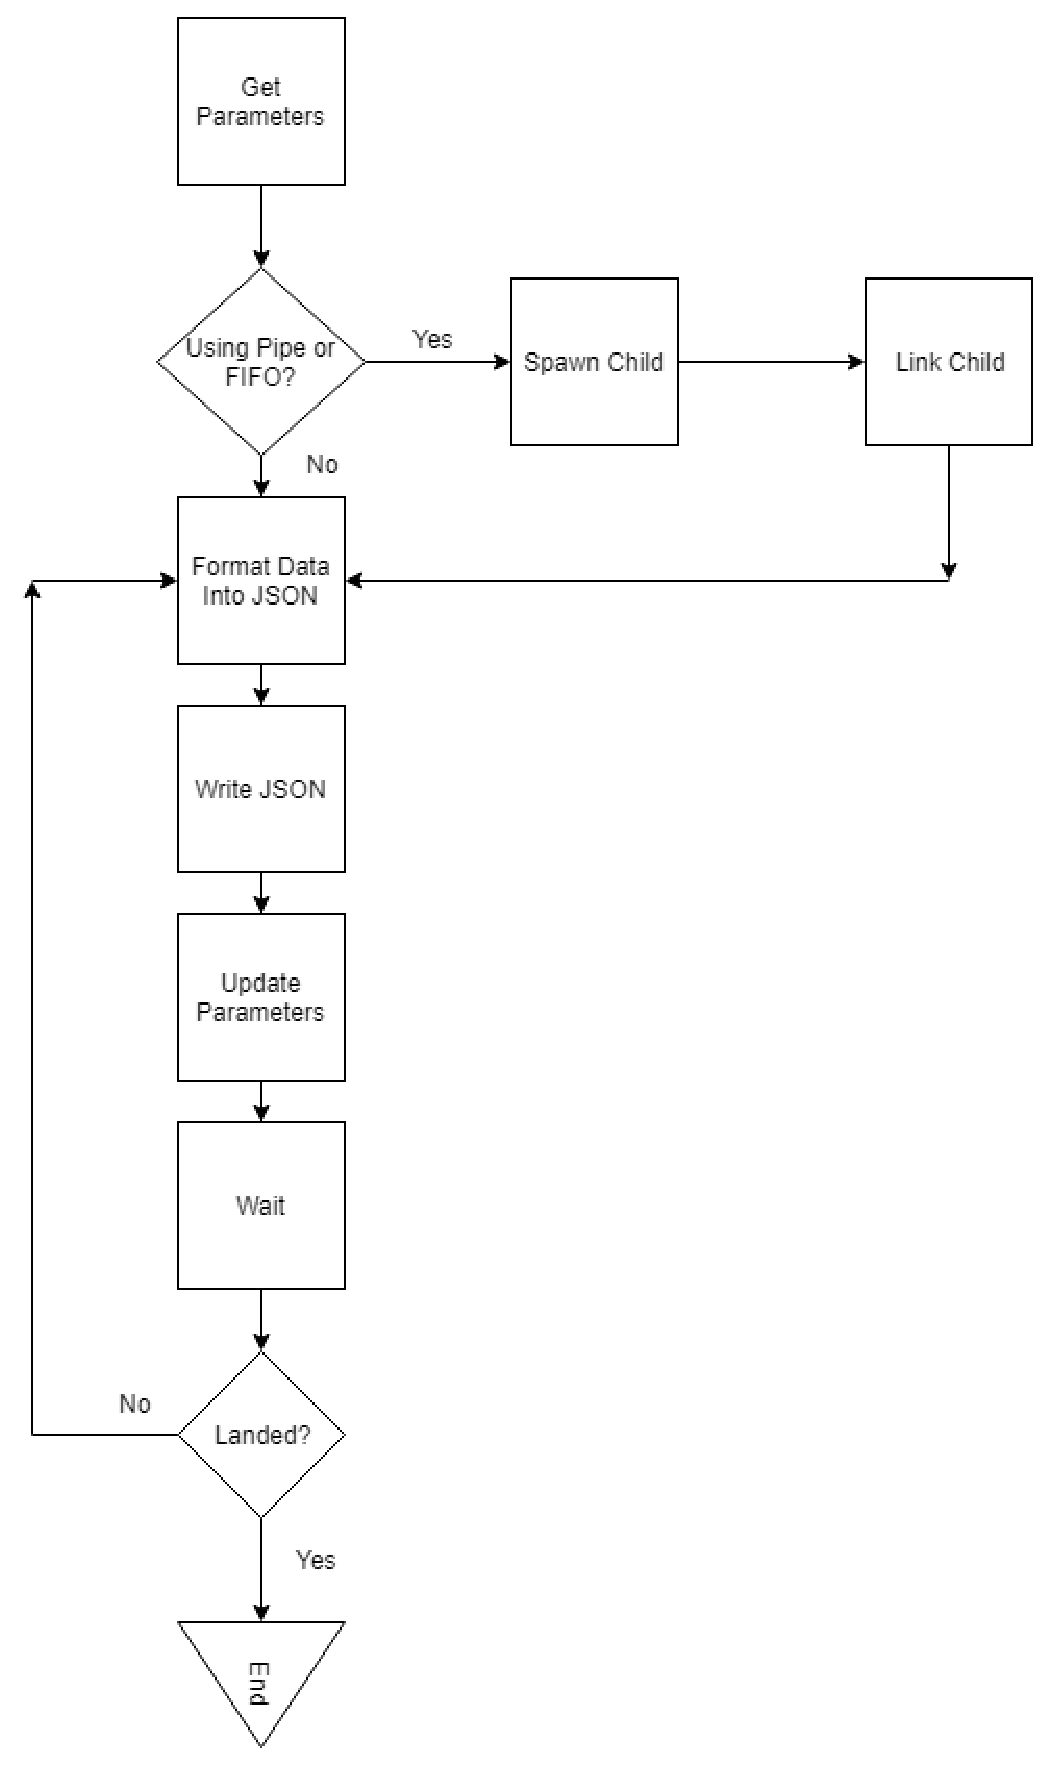
\includegraphics[height=8cm]{datagen}
        \caption{Design for data generator}
        \label{fig:datagen}
%    \end{subfigure}
\end{figure}

\subsubsection{Instructions}
To run the user should first navigate to the data\_generator directory. Once there the generator can be started with ./gen. There are several command line arguments that can change functionality. The –vel flag allows changing of initial velocity, the –lat and –lon arguments allow changing of initial latitude and longitude. The –alt allows the setting of the initial altitude. The – type followed by b or s will set the type as booster or sustainer for the JSON string output. The –rate option changes the frequency with which data is generated. The –pipe option followed by the command to run another program allows the program to spawn a child process and send it data via a pipe, received on file descriptor three, or using -pipeno the user can change the file descriptor. The –fifo argument does the same thing except with a FIFO instead of a pipe. The –test flag seeds random in a specific way such that all random data will be the same with each running with this option enabled. The –debug flag gives out extra information about the internal system. The – to flag sets the file to write to if not using a pipe or FIFO. The final options are the –buff and –wind flags to set the read buffer size for logger as a sub process, and to set extra variance to a certain direction of the simulated data. These are both old and it is not suggested that they ever be used.
\subsubsection{Testing}
The data generator is meant to be a testing module for the rest of the system, so it had to work flawlessly. Most of the testing was done manually, where the developer would change parameters and make sure that each response was in the correct JSON format. After that the JSON was tested by trying to use the JavaScript jsonify function to better ensure that the data was being formatted correctly. The data was later tested by pushing it to the database and having each return a success, proving that the data was coming in a format expected by later portions of the system.
\subsection{Data Handling}
\subsubsection{Requirements}
The only requirements the data handling system needs to run are a Linux operating system and C++ compiler. The system however consists of several parts and other than the test system, will require either the custom PCB created for this project by the Electrical Engineering team, or an Altus Metrum Teledongle and Telemega. These are the sensor packages used to retrieve the real data, and this system can only use test data without them. The system is installed with the above installation instructions.
\subsubsection{Design}
The system in essence is a state machine, using FIFOs to enforce timing. The system does initial system setup, such as making pipes and FIFOs and spawning child processes, then begins a loop. The loop waits for data from the booster FIFO then from the sustainer FIFO, if the Boolean that says they are completed is false, if the data retrieved was the end of transmission signal then the Booleans are set and they are no longer checked. Then any retrieved data in sent to the loggers via pipes and to the database API via their respective FIFOs. Then after both end it breaks the loop and does cleanup, such as closing files and waiting on all its child processes, and ends.
\subsubsection{Instructions}
To run the system the user must have four separate terminals open. The first must be in the data\_handling directory, and the user must run ./start\_docker\_with\_erase.sh to begin a new docker instance and erase all previous data from old runs. If Docker was already running they should run ./stop\_docker first. Then on the second terminal also in the same directory the user will run ./datahandle. Finally on the other two screens the user decides the source of data, The easiest to to run a test, where the user types ./gen –type b > b\_data\_fifo, and on the remaining screen runs ./gen –type s > s\_data\_fifo. This will run a test of the system with two data generators. The other option is to run two instances of PUTTY gathering data from the serial ports upon which the receiver boards are connected from the Electrical Engineering project, and then run those through another FIFO into the converter.py process and then output that into the b\_data\_fifo and s\_data\_fifo. The last option is to do the same, except for the Teledongle is the source of incoming data and instead of the convert.py process the user uses the tr\_s and tr\_b processes to convert Teledongle packets on Telemega data and convert these packets into JSON packets which the data handler can utilize. The data handler does not care how it gets the data, it just requires that it comes in from the expected JSON format and the booster data comes in from the b\_data\_fifo and the sustainer data comes in from the s\_data\_fifo.
\subsubsection{Testing}
Testing was done by linking the system to the already well established data generator and running several simulations. Each simulation had to display a reasonable graph of the data through the web application, implying it was correctly pushed to the database, as well as record the data into two log files with matching data points. Stress tests were used to prove that the system could keep up with a rate as high as 100 packets a second, which was far higher than the once per second that was expected.
\subsection{Translation}
\subsubsection{Requirements}
The translate modules do not require anything more than a Linux operating system and a C++ compiler. However this is only to make the programs correctly. They are useless without the Teledongle and A connected Telemega, as the purpose of these processes is to convert the Telemega data into JSON data that can be used later on my the system. To compile them, be in the data\_handling directory and type g++ translate\_s.cpp –o tr\_s then g++ translate\_b.cpp –o tr\_b. This will compile them correctly if you have g++ installed and you are on a Linux operating system.
\subsubsection{Design}
The design for these systems is simple. They open a file and then read a single line at a time as long as they can, then they take this line and parse it for the packet identifier. If the identifier indicates it is a GPS packet then it uses the hard coded offsets to get the correct sub strings and converts them into numbers and does any required math to get the true value. Then the data is formatted into a JSON string and written to the screen. The following figure displays the design.
\begin{figure}[h]
    \centering
%    \begin{subfigure}[Figure 1a]{0.3\textwidth}
        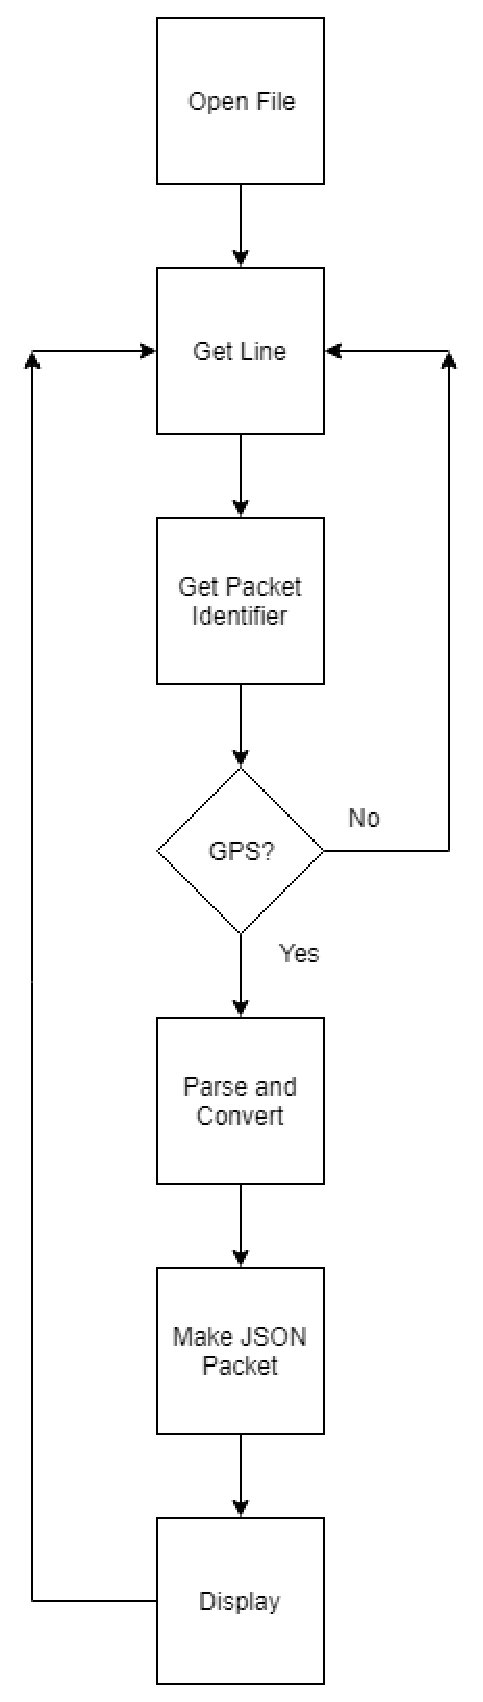
\includegraphics[height=8cm]{Translate}
        \caption{Translation design}
        \label{fig:Translate}
%    \end{subfigure}
\end{figure}

\subsubsection{Instructions}
To run wither the user must be in the data\_handling directory and run ./tr\_s for the sustainer and ./tr\_b for the booster. The user must also enter a –file flag followed by a file name to indicate where the process will collect data from. Then the user must use a –post flag if the data is being read from a log after the fact to add a 1 second delay between conversions.
\subsubsection{Testing}
The testing was done by linking the translator to a data stream coming in from a Teledongle Hooked up to a Telemega at the test launch in Brothers, Oregon. The data was recorded and then sent through the system several times afterwards. The data created confirmed that the altitude, latitude, and longitude were all at the correct values as expected by comparing these results to the industry made AltOS.
\subsection{3D Trace}
\subsubsection{Requirements}
The 3D trace created for this project can only run in a specific environment. Any attempt to run this program in any other environment is not guaranteed to produce correct functionality. More specifically the system was wholly developed and tested on one laptop, which was determined to be the ground station for the project and thusly was the only system upon which the system needed run. It is expected, however, that the system should function properly on any Linux system with a C++ compiler and OpenGL installed regardless of processor or graphics accelerator, but again, this is not a guarantee. The system is installed by the instructions described above and require no extra steps for installation.
\subsubsection{Design}
The system runs off of OpenGL via a C++ interface. OpenGL is an API for accessing the graphical capabilities of a hardware graphics accelerator. It is in essence a large state machine that updates as frequently as it can to display the newly rendered image to the display adapter. This particular interface was chosen for its widespread availability as well as the experience available both within the team as well as from mentors at the university.
There are two modes is which the trace may run, postflight and near real time (NRT). These have slightly different sequences of operation. The post flight mode and NRT mode share detection of Internet, detection of arguments, and initial setup for the graphics subsystems. The NRT mode then initializes its latitude and longitude. Both then initialize common geometry. Here is where the post flight mode retrieves its data from a file and then creates the flight path representation. Both then create a map from the Google static maps API if there is an Internet connection or decide to use the default map. Both then initialize textures. Both continue to initialize more graphical and logistical sub-systems, and both begin the main display loop, which executes until the program is exited. The NRT mode will at a rate of sixty times per second retrieves data from a pipe and then converts it into a new data point and updates the geometry for the flight path. The design can better be seen in the following figure.
\begin{figure}[h]
    \centering
%    \begin{subfigure}[Figure 1a]{0.3\textwidth}
        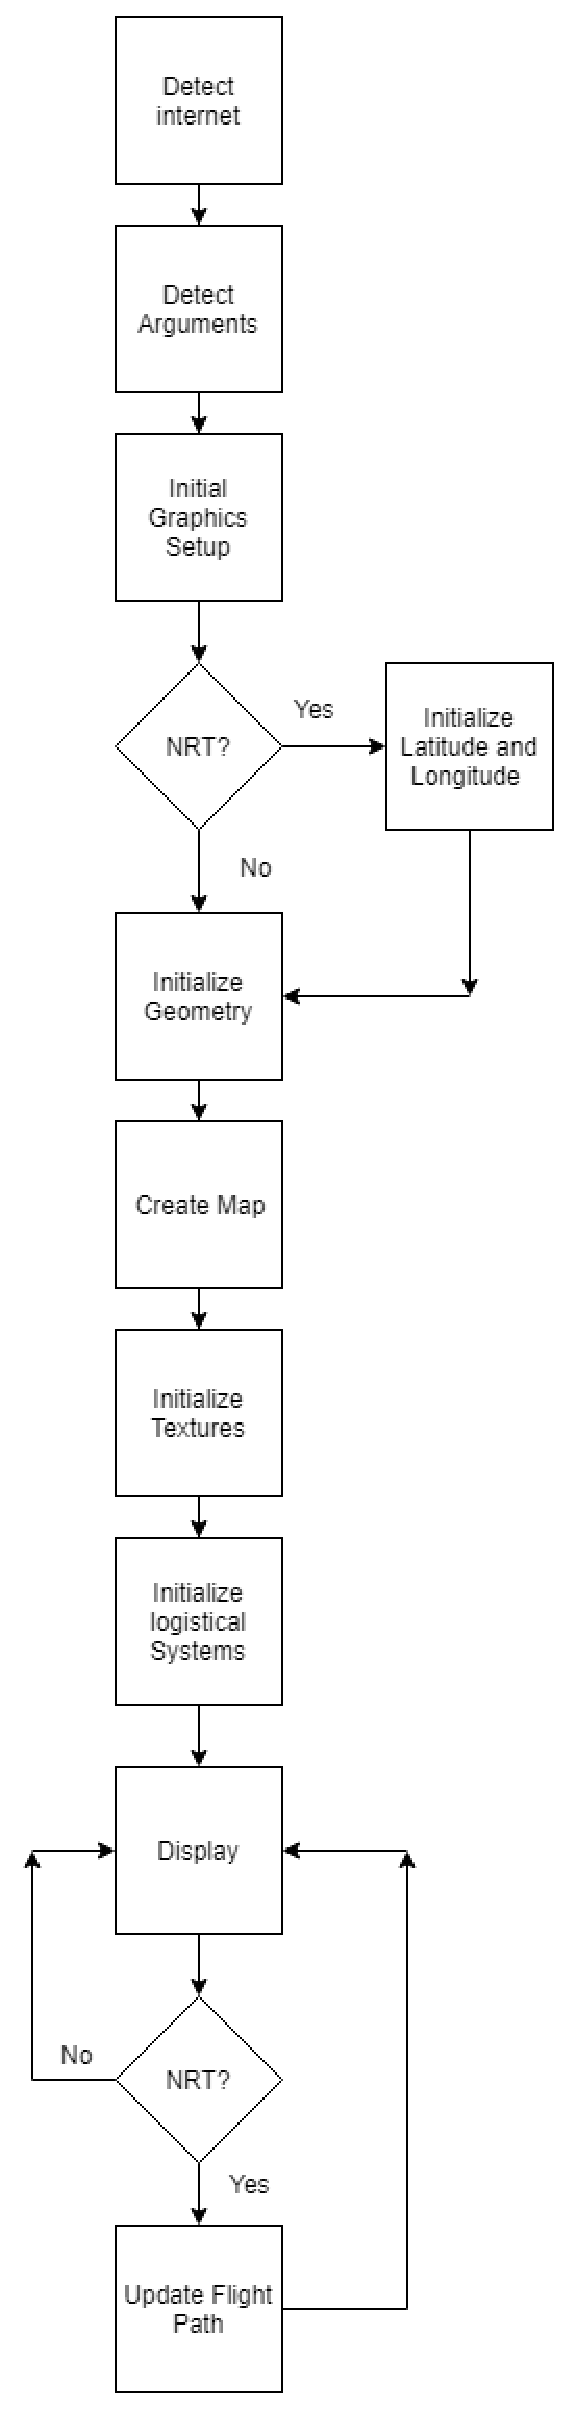
\includegraphics[height=8cm]{trace}
        \caption{Overview of trace design}
        \label{fig:trace}
%    \end{subfigure}
\end{figure}

\subsubsection{Instructions}
To run in a post flight mode, put the log file you wish to display into the same directory as the executable for the trace which should be 100kRocketryAvionics2017-18/3d\_trace and name it log.txt. Then you simply run ./trace. For post flight mode the data must be taken from a source program and piped through to the trace as a child process with file descriptor three used as the communication file. It is suggested that this is not attempted manually. To see this in action one can try while in the same directory as the trace executable, run ./gen -vel 1000 -rate 60 -pipe ./trace -nrt. This is a test of the NRT mode using the data generator. The NRT mode is operational, but not often used, as this aspect had never been a system requirement, and the inter operation with the data handling side was not finished due to time constraints.
There are a few arguments that can be used to modify operation. The -nrt flag indicates NRT mode is to be used. -x followed by a number is the scale in the x direction. The -y flag followed by a number indicates the scaling in the y direction. The -z flag followed by a number indicates the scaling in the z direction. The -center flag will center the flightpath at the origin in post flight mode. \par
When in operation there are a few things that can be done. Holding a left mouse button and moving it will rotate the scene. The middle mouse button will allow zooming in and out. The a, s, w, and d keys will allow for panning and zoom depending on rotation.
\subsubsection{Testing}
The system primarily needed to be user tested, as it is graphical in nature. The technical requirements were that it displayed the scene in the expected way, so the developer would compile and run with every change to make sure that the scene displayed properly. The conversion from latitude and longitude to miles was tested by using the –debug flag when running the trace to print out the distances from the origin, and then comparing those with the values returned for the same data from the National Hurricane Center.

\subsection{Web Application and Database Structural Overview}
The web tools component of this project is comprised of a REST API, web application and database. These components all work together in order to effectively gather, manipulate and display critical telemetry related to the rockets flight. The following is a diagram which details how each module interfaces with one another.
\begin{figure}[h]
    \centering
%    \begin{subfigure}[Figure 1a]{0.3\textwidth}
        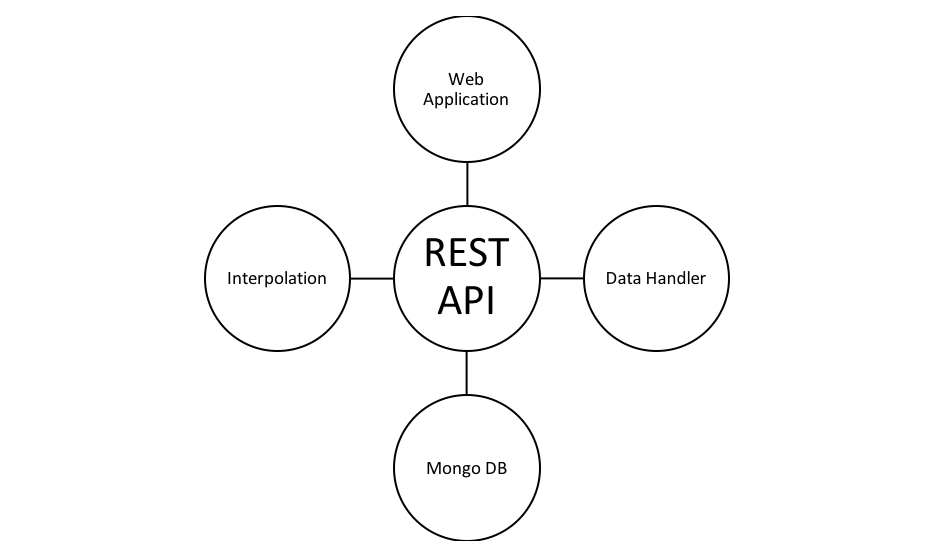
\includegraphics[height=8cm]{module_integration}
        \caption{Module integration with REST API}
        \label{fig:module_integration}
%    \end{subfigure}
\end{figure}

\subsection{Installing the Web Application, Web API, and Database}
Each component of the web tools suite has a respective docker container that has the required dependencies for each tool. This makes the installation and configuration portion of the project fairly straight forward. As the software will be running in containers this means as long as one has Docker installed on their base system and have virtualization capabilities then running the web tools software suite is not a problem. To bring the web suite into a running state one must ensure Docker with Docker compose is installed on their system, navigate to the web tools directory in the git repository and finally run “docker-compose up”. This will standup three containers “web\_tools\_app”, “web\_tools\_api” and “web\_tools\_db”. “web\_tools\_app” will have port 8080 exposed in order to access the web application from the host machine web browser and “web\_tools\_api” will have port 5000 exposed in order to make API requests from outside of the Docker networking environment. For example, tools such as the data handler and data generator which live outside of the Docker environment take advantage of the REST API to send and receive data. In addition to ports being exposed some directories from the host machine are directly mapped to the container environments. Relative to the git repository, the application data is stored in ./app and will map to /app in the “web\_tools\_app” container. The REST API application data is stored in ./api and will map to /api in the “web\_tools\_api” container. The purpose of making these volume mappings for the app and REST API tools is to sync any updates to source code to related containers. Lastly another volume mapping is created for the database container. This mapping is required in order to persist data between each re-instantiation of the database container. 
\subsection{Utilizing Web Application and Web API}
Once the installation instructions have been followed and the three web tool containers are running without issue it’s now possible to run the web application and REST API. The web application has one endpoint “/” and is accessible via the host machine using the IP address of the local machine. e.g. “localhost:8080/” This will take you to the main interface for the web application. Here you will have access to the flight chart information which displays altitude for both the booster and sustainer stages over time. This chart is located on the top left of the web application and each curve is color coded blue for the sustainer and orange for the booster. This widget provides good insight into how the rocket handled throughout flight. Some events that can be determined from this data include when the booster separated from the sustainer which is identified as a separation between each curve. Another event that can be determined by the web interface is whether the parachutes assisted with the landing of both stages of the rocket. This should be clear in the rate of change of acceleration over time. If one or both of the curves were to sharp gradients, then it is likely the parachutes didn’t slow the stages down correctly or they were not deployed entirely. Just under the altitude flight chart in the interface contains the sustainer and booster GPS cards. These cards are used to display and update GPS data for both sections every second. The GPS data is a tuple of latitude and longitude coordinates. This information is useful for tracking each stage of the rocket throughout its flight. On the top right of the interface there’s a card that indicates stage and duration of the flight. This card calculates the duration of flight based on the time value that was set during the first stage of the data handler execution. This is a useful feature because this will indicate how long the rocket has been in flight and which stage of flight the rocket is in. Just below the stage and time duration card are the altitude and speed gauges for both the sustainer and the booster. These gauges will update a frequently as data is received from the database. This feature will allow one to view the speed and altitude of each stage at a given time. The default units of measurement for each section are miles per hour for speed and miles for altitude. This option is configurable within the code but not available for manipulation on the web interface. This is something that could be integrated at a later date. As standard this allows the user to get a good idea of what is going on with the rocket throughout its flight. That concludes an explanation of how to run and interface the web application. \par

The REST API has nine endpoints, and all are accessible via the host machine using the IP address of the local machine. e.g. “localhost:8080/” or from the other docker containers using the IP address of the “web\_tools\_api” container. The most useful tool for accessing and testing this REST API is “Postman” which is a free tool to test APIs. The routing convention for the REST API is as follows: ``HOSTNAME:5000/api/<version\_\#>/endpoint'' The current version of this API is “v1.0”. \par

The “get\_all\_telemetry” endpoint is accessible via “HOSTNAME:5000/api/v1.0/telemetry\_all” and supports the GET method only. The purpose of this endpoint is to supply all related telemetry for both the booster and the sustainer since the beginning of the rocket launch as one large JSON dictionary. This JSON dictionary is order from most recent data to oldest. \par

 The “get\_telemetry” endpoint is accessible via “HOSTNAME:5000/api/v1.0/telemetry/<t\_type>” and supports the GET method only. <t\_type> is variable provided to determine which stage one requires telemetry from. “get\_telemetry” is responsible for only returning the latest telemetry packet from a specific stage on the rocket. \par

The “prepare\_launch” endpoint is accessible via “HOSTNAME:5000/api/v1.0/prepare\_launch” and supports the GET method only. The purpose of this endpoint is to create a launch document in the database and return the document id for later manipulation of launch data.\par

The “get\_launch” endpoint is accessible via “HOSTNAME:5000/api/v1.0/launch” and supports the GET method only. The purpose of this endpoint is to provide “start\_time” and “end\_time” data related to the launch. \par

The “start\_launch” endpoint is accessible via “HOSTNAME:5000/api/v1.0/start\_launch/<launch\_id>” and supports the GET method only. The <launch\_id> is a variable provided to verify for which launch the start time should be logged for. The purpose of this endpoint is to set a timestamp value in the database for when the rocket was launched. \par

The “end\_launch” endpoint is accessible via “HOSTNAME:5000/api/v1.0/end\_launch /<launch\_id>” and supports the GET method only. The <launch\_id> is a variable provided to verify for which launch the end time should be logged for. The purpose of this endpoint is to set a timestamp value in the database for when the rocket has landed. \par

The “post\_telemetry” endpoint is accessible via “HOSTNAME:5000/api/v1.0/telemetry >” and supports the POST method only. The purpose of this endpoint is to insert new telemetry into the database. This could be from the data\_handler or from the data\_simulator. Here’s an example telemetry packet that could be posted to the database via this endpoint:
{"velocity":"100.000000", "latitude":"45.000000", "longitude":"45.000000", "altitude":"0.000000", "time":"0.000000", "type":"s"}. Where velocity, latitude, longitude, altitude and time are floating values and type is a character value. \par


The “interp\_telemetry” endpoint is accessible via “HOSTNAME:5000/api/v1.0/interp\_telemetry” and supports the POST method only. The purpose of this endpoint is add telemetry that has been interpolated to a separate collection called interp\_telemetry which can be used to get an estimate on the trajectory of the rocket. \par


The “remove\_all\_data” endpoint is accessible via “HOSTNAME:5000/api/v1.0/cleardata” and supports the GET method only. The purpose of this endpoint is to remove all data within the database. This includes launch data and telemetry data. This endpoint should be used with caution and should only be made available when in testing environments. \par

\section{Recommended Technical Resources}
The following list enumerates several resources that aided in project development. They may prove useful in similar projects or for furthering understanding of the topics pertinent to this project. 
\begin{enumerate}
   \item AltOS Telemetry: https://altusmetrum.org/AltOS/doc/telemetry.html
   \item Opengl.org: https://www.opengl.org/
   \item Cppreferance.com: http://en.cppreference.com/w/
   \item Latitude/Longitude Distance Calculator: https://www.nhc.noaa.gov/gccalc.shtml
   \item Flask: http://flask.pocoo.org/docs/1.0/
   \item MaterializeCSS: https://materializecss.com/
   \item MongoDB: https://docs.mongodb.com/manual/
   \item Docker: https://docs.docker.com/v17.09/
   \item Python: https://docs.python.org/3/index.html
   \item Postman: https://www.getpostman.com/docs/v6/
   \item GPS Information from NMEA: http://www.gpsinformation.org/dale/nmea.htm
   \item OpenGL Programming Guide Ninth Edition ISBN-13: 978-0134495491
   \item The C programming Language Second Edition ISBN-13: 978-0131103627
   \item Dr. Mike Bailey at Oregon State University.
   \item Benjamin Brewster at Oregon State University.
   \item Keith Packard from Altus Metrum.
   \item JPL C Coding Standard
   \item An Introduction to the Kalman Filter - Greg Welch and Gary Bishop
   \item Wikipedia page for Kalman Filter
   \item Elementary Numerical Analysis, 3rd Edition by Kendall Atkinson and Weimin Han
\end{enumerate}

\section{Conclusions and Reflections for Michale Elliott}
During this project I learned a lot about different processes used in the computer science world.
The main concepts I learned about were filtering, interpolation, and extrapolation.
I also learned about meeting strict C standards for my embedded code and improving compatibility with obscure hardware.
The linear algebra used in the Kalman Filter was certainly outside of my comfort zone prior to the project, and I am much more confident in my abilities now.
While the numerical analysis required for this project was material I had covered in a class previously, I had not had the opportunity to make an application surrounding the concepts.
For the interpolation module I learned about programming custom python modules in C which will prove very useful in the future.

I did not learn much about project work that I did not already learn from working as a developer, but I did learn a lot about self-led projects.
The project was pretty free-form, and although there were a few deadlines set in class and by the client, most of the development deadlines had to be set by ourselves.
This was quite different from having a deadline for a project set by a boss or a professor, and I learned a lot about time management.
I also learned a lot about people management and working together with others.
I was fortunate enough to have quality team mates that did all of their work, but it was still sometimes a struggle to coordinate two or three meetings per week with our busy schedules.
We also spent a lot of time making sure our code worked together, which is more difficult when everyone is working on their own part of the project.
This led to a couple of git merges that would have been issues if we hadn't worked together to fix them.

Many of the issues we encountered throughout the term were with hardware and firmware, so if I were to do this project over again I would likely spend more time making sure that all came together better.
I would also do more testing to prove the correctness and robustness of the code because, while we did do testing of the code, we could always have done more.
For the Kalman Filter, I had originally planned on having a complex system of error handling to improve the robustness of the program, but I ended up not having enough time to implement it before we had to do beta testing.
I also found a better solution than a Kalman Filter that was written up in a recent paper that would have been easier to implement.
Unfortunately I did not find this solution until we were too far along in the project.
Finally, while mostly a non-issue, I sometimes confused the names of similar technologies or methods, which can appear sloppy.
\section{Conclusions and Reflections for Samuel Hudson}
Throughout this project I was able to learn a lot about web service development and non-monolithic architecture techniques. The requirements of this project called for a web application with a database and REST API. It was interesting to see how each component integrated with one another using the REST API. This is something I have never tried in practice. The API acts as a layer of abstraction between each sub-component making integration trivial. I would also say that my python programming skills have also strengthened throughout this course. \par
One of the most important non-technical skills I learned from this project was effective time management. This was very important because there were many deadlines and meetings that had to be met. Often, I would find myself planning ahead to ensure everything was in order for upcoming meetings and deadlines. Having an idea of time was critical to ensure the success of the project. \par
Project work has its advantages and disadvantages. Some of the advantages include the distribution of workload, more people to think through problems and greater levels of combined experience. Working in a team made the it easy to work through the larger problems such as developing the data generator and syncing with the rocket during flight. Some of the disadvantages included the weakest link component. For example, if someone in the group had not completed their work that was integral in another component this can cause delays and negative consequences. \par
Project management ties into a lot of skills I’ve learned surrounding time and task management. The project’s success is dependent on things being completed in a timely manner and everyone contributing their part. Planning was a big part of the project management process. Ensuring that there was a plan for each of our development efforts was crucial. \par
Teams make it easier to tackle problems because people think differently and provide different levels of experience. In my opinion the combined experience of a team is much more powerful than the experience of an individual alone. There are some benefits to working as an individual such as not having to coordinate with other people which can take time. \par
If I was to do it all over again one of the main changes I would have made is to the web interface. Although MaterializeCSS is a good front end framework it wasn’t as visually enabling. I would most likely use Kibana next time. Kibana is an open source framework that provides a more vibrant interface. Another change that I would make is to the way that information was gathered from the API. In the future I would like to see the web application use sockets instead of just polling the endpoint for new data. This means that each time there was an update to the database an update would be sent to the web application. This would have been a more efficient method for sending data to and from the web application and database. Another change I would make to the web interface is allow the user to select which units the gauges would work in. For example, the user could select feet per second instead of miles per hour for speed. Lastly, I would like to have the web suite hosted outside of the local machine. This would make the application much more accessible. \par

\section{Conclusions and Reflections for Glenn Upthagrove}
During the course of this project I learned a few technical skills. I learned most of all how to better write embedded C, and I learned much more about the ARM architecture. However I learned very little new on the software side of for my main portions of the project. This is not to say the experience was not useful, as I relearned and in some cases for the first time applied how to properly use several different tools and skills I had learned or heard about but had not used or had used very sparingly in the past. These include the use of usleep, FIFOs, and pipes. I also learned a lot about Python and some of its libraries that I had never used before. I did learn much more about GIT and I also learned how to use a little of Travis CI. \par
I learned a lot more on the non-technical side of this project. I learned a lot about intra and inter team correspondence, I learned a lot about project management tools, and I learned how to work with and converse with people in fields outside of my own much better. This project being as large and diverse as it was probably was one of the best in this year’s selection when it came to learning more about how multidisciplinary projects work, and how to handle the challenges of meeting the needs of and waiting on the progress of other disciplines. I also learned that conflict is sometimes unavoidable, and is sometimes a good thing for getting the flow of work moving forward again. I also learned that these situations can be resolved peacefully and mitigated, most especially if they are caught early and if the proper communication follows. Teams will have good and bad days, and the makeup of the team is important. If the team does not get along the work will suffer, and if they do the work may exceed expectation. This is not to say that personal accountability can be written off to the coherence of the team. Many of these can be mitigated by larger efforts on the part of the individual. While each person is not on their own capable of resolving all matters, they can aid in their resolution and nothing replaces the personal accountability of each team member. Teams comprised of multiple disciplines such as ours was are even harder to continuously maintain and keep track of. This is why regular and honest communication is paramount in the success of this paradigm. Good project management is important and requires good communication. Project management can also be aided by the utilization of the proper tools. While all members of our computer science team were able to and often did aid the others with their work, the even dividing of workload was very important in the success of the project, and also to give the jobs to the member most skilled in that area. There is no harm in letting and individual’s skills shine and the work will be better for the proper utilization of that person’s talent and experience.\par
I would have to say if I could do this entire project over again I would not do it the same way. There are several things I think could have been approached in a better way from the start. Team management and division of labor could have been more clearly set up and distributed much earlier on in the process, both inside and outside the computer science team. The responsibilities of each individual sub team and each individual person were not as clear as they should have been from the start and that led to several instances of uneven divisions of labor or last minute additions to requirements. I think if this had been better planned this would not have happened. Also responsibilities were not always correctly handled by the person or team who was supposed to be assigned to that requirement. I think many of our technical work was done in a good way, and I would not change the back end of how most of the system works. The only technical thing I would argue for the change of is better scripting of work for the data handling. This is due to heavy delays brought about by hardware, and thus a rushed development cycle on these parts, however that does not change the fact that it makes them difficult to use. The hardware issues should have been resolved much earlier, and then the software that handled the data should have been given a higher priority. They user, if I could rebuild the system, would never even need to worry about typing, but could instead hit the button in a GUI that would then start a binary that would take care of all the messy details of data handling form them. Overall I would say that whilst the system works perfectly well, there are ways in which it could have been improved had the project been gone about in a different manner.
\section{Appendix A}
\subsection{NMEA Extract}
Here is an extractor for NMEA GPS data.
\begin{lstlisting}
struct gps_data extract_nmea(char data[])
{
    const char s1[2] = "\r";
    const char s2[2] = ",";
    char *token1, *token2;
    char *saveptr1, *saveptr2;
    token1 = strtok_r(data, s1, &saveptr1);
    char des[80];
    struct gps_data r;
    while (token1 != NULL)
    {
      strcpy(des, token1);
      token2 = strtok_r(des, s2, &saveptr2);
      const char *t[15];
      int i = 0;
      if (strncmp(token2, "$GNRMC", 7) == 0)
      {
        while (token2)
        {
          t[i] = token2;
          token2 = strtok_r(NULL, s2, &saveptr2);
          i++;
        }
        i = 0;
        if (strncmp(t[2], "A", 2) == 0)
        {
          r.lat = atof(t[3]);
          r.lon = atof(t[5]);
        }
        else
        {
          r.lat = 0.0;
          r.lon = 0.0;
        }
      }
      else if (strncmp(token2, "$GNGGA", 7) == 0)
      {
        while (token2)
        {
          t[i] = token2;
          token2 = strtok_r(NULL, s2, &saveptr2);
          i++;
        } 
        i = 0;
        r.alt = atof(t[9]);
      }
      token1 = strtok_r(NULL, s1, &saveptr1);
    }
    return r;
}
\end{lstlisting}
\subsection{How to make a set of data}
Below is how data can structured into the expected format for this system.
\begin{lstlisting}
/***********************************************
*Title: structure
*Params: a string pointer
*Description: Converts a JSON packet into a
*telem_data structure
***********************************************/
struct telem_data structure(char** buff){
        char* messagecpy;
        char* token;
        struct telem_data data;


        token = (char*)malloc(sizeof(char)*256);
        messagecpy = (char*)malloc(sizeof(char)*256);
        memset(token, '\0', 256);
        memset(messagecpy, '\0', 256);
        strcpy(messagecpy, *buff);
        token = strtok(messagecpy, ":");
        token = strtok(NULL, "\"");
        data.vel = atof(token);
        token = strtok(NULL, ":");
        token = strtok(NULL, "\"");
        data.lat = atof(token);
        token = strtok(NULL, ":");
        token = strtok(NULL, "\"");
        data.lon = atof(token);
        token = strtok(NULL, ":");
        token = strtok(NULL, "\"");
        data.alt = atof(token);
        token = strtok(NULL, ":");
        token = strtok(NULL, "\"");
        data.time = atof(token);
        token = strtok(NULL, ":");
        token = strtok(NULL, "\"");
        data.type = token[0];
        return data;
}

#endif
\end{lstlisting}
\subsection{Installation}
Below is the installation script for the system.
\begin{lstlisting}
echo "installing apt-file"
echo
sudo apt-get install file -y
sudo apt-get install apt-file -y
echo
echo "updating apt-file"
echo
sudo apt-file update -y
#docker
echo
echo "installing docker" 
echo
sudo apt-get install docker.io -y
sudo apt-get install docker-compose -y
#C/C++
echo
echo "installing gcc" 
echo
sudo apt-get install gcc -y
echo
echo "installing g++" 
echo
sudo apt-get install g++ -y
#Make/CMake
echo
echo "installing make" 
echo
sudo apt-get install make -y
echo
echo "installing cmake" 
echo
sudo apt-get install g++ cmake -y
#OpenGL
echo
echo "updating" 
echo
sudo apt-get update -y
echo
echo "upgrading"
echo
sudo apt-get upgrade -y
echo
echo "installing mesa-utils" 
echo
sudo apt-get install mesa-utils -y
echo
echo "installing mesa-common-dev"
echo
sudo apt install mesa-common-dev -y
echo
echo "installing freeglut"
echo
sudo apt-get install freeglut3 -y
sudo apt-get install freeglut3-dev -y
sudo apt install libglu1-mesa-dev freeglut3-dev -y
echo
echo "copying libglut.so to /usr/lib64"
echo
sudo mkdir /usr/lib64
sudo cp ./3d_trace/libglut.so /usr/lib64/
sudo chmod o=rwx /usr/lib64/libglut.so
sudo chmod u=rwx /usr/lib64/libglut.so
echo
echo "installing binutils-gold"
echo
sudo apt-get install binutils-gold -y
echo
echo "installing libglew"
echo
sudo apt-get install libglew-dev -y
echo
echo "installing build-esssential"
echo
sudo apt-get install build-essential -y
echo
echo "installing libglew 1.5 dev"
echo
sudo apt-get install libglew1.5-dev libglm-dev -y
#Python and required modules
echo
echo "installing python"
echo
sudo apt-get install python -y
echo
echo "installing pip" 
echo 
sudo  apt-get install python-pip python-dev build-essential -y 
sudo  pip install --upgrade pip 
sudo  pip install --upgrade virtualenv 
echo
echo "installing Pillow module for python"
echo
sudo pip install Pillow
echo
echo "installing requests module for python"
echo
sudo pip install requests 
echo
echo "installing pyUSB"
echo
sudo pip install pyusb
echo
echo "updating"
echo
#update and upgrade
sudo apt-get update -y
echo
echo "upgrading"
echo
sudo apt-get upgrade -y
echo
echo "Done"
echo
#make
echo
echo "Making programs"
echo
cd 3d_trace
make
cd ..
cd logging
make
cd data_handling
make
cd ..
cd data_generator
make
cd ..
cd conversion
make
cd ..
echo
echo "done"
echo
#make desktop icon
echo
echo "making desktop icon"
echo
cp ./HART.desktop ~/Desktop
echo
echo "Done"
echo
echo
echo "Creating Directory File"
echo
pwd > HART_DIR.txt
sudo mv HART_DIR.txt /HART_DIR.txt
echo
echo "Done"
echo

\end{lstlisting}

\subsection{Divided differences formula}
Below is the formula for divided differences used in the Lagrange interpolation formula.

\begin{lstlisting}
def interp_coeffs(data):
        n = len(data)
        xvals = [x for x, y in data]
        yvals = [y for x, y in data]
        diff = []
        for i in xrange(n):
                diff.append([0 for j in xrange(n)])
                diff[-1][0] = yvals[i]

        for i in xrange(1, n):
                for j in xrange(i, n):
                        diff[j][i] = (diff[j][i-1] - diff[j-1][i-1]) / (xvals[j] - xvals[j-i])

        return [diff[i][i] for i in xrange(n)]

\end{lstlisting}

\bibliographystyle{IEEEtran}
\bibliography{bibliography}
\end{document}
